\setTopic{Sets and Functions}
\setAuthor{M. Andrew Moshier}
\setDate{October 2014}
\setCourse{Discrete Mathematics}

\setOverview{
The mathematical universe consists of various things: numbers, functions, graphs, lists and so on.
A \noexpand\emph{set} is collection of things. 
For example, the collection of all natural numbers is a set.
A \noexpand\emph{function} is a correlation of the members of one set with members of another set.
These two abstract concepts (sets and functions) form a conceptual framework in which virtually all of mathematics can be built.
So an understanding of sets and functions is key to a rigorous approach to most other parts of mathematics.
This conceptual framework can itself be put on a formal, precise footing called the Category of Sets and Functions.
In these lectures, we investigate the Category of Sets and Functions, so that we can use these things as the basic building blocks of everything else we do.
}

\chapter{Sets}

\begin{goals}
\noindent\textbf{Lecture}
\begin{itemize}
\item Describe informally the category of sets.
\item Define list set notation.
\item Introduce the idea of a subset.
\item Introduce the axiom of extensionality for sets and some of its consequences.
\end{itemize}

\noindent\textbf{Study}
\begin{itemize}
\item Demonstrate ability to determine equality of sets.
\item Develop facility in basic set theoretic notation.
\end{itemize}
\end{goals}

\emph{Sets} are the mathematician's way of thinking about \emph{collections} of objects. Examples will be the set of natural numbers, the set of pairs of natural numbers, the set of real numbers, and so on.

An example is a set representing poker cards. We may denote it by
\begin{align*}\symb{Deck}=\{&A\clubsuit,2\clubsuit,3\clubsuit,4\clubsuit,5\clubsuit,6\clubsuit,7\clubsuit,8\clubsuit,9\clubsuit,10\clubsuit, J\clubsuit,Q\clubsuit,K\clubsuit,\\
&A\diamondsuit,2\diamondsuit,3\diamondsuit,4\diamondsuit,5\diamondsuit,6\diamondsuit,7\diamondsuit,8\diamondsuit,9\diamondsuit,10\diamondsuit, J\diamondsuit,Q\diamondsuit,K\diamondsuit,\\
&A\spadesuit,2\spadesuit,3\spadesuit,4\spadesuit,5\spadesuit,6\spadesuit,7\spadesuit,8\spadesuit,9\spadesuit,10\spadesuit, J\spadesuit,Q\spadesuit,K\spadesuit,\\
&A\heartsuit,2\heartsuit,3\heartsuit,4\heartsuit,5\heartsuit,6\heartsuit,7\heartsuit,8\heartsuit,9\heartsuit,10\heartsuit, J\heartsuit,Q\heartsuit,K\heartsuit\}
\end{align*}
The elements are arranged here conveniently, but we could just as well have listed the cards in any ``shuffled'' order. The set of them would be the same.

\emph{Functions} are the mathematicians way of thinking about attributes of the things in a collection, like ``the color of'', ``the mass of'', ``the location of'', ``the father of'', ``the favorite book of the person to the left of'' and so on.
For our example of cards in a poker deck, ``rank of'' or ``suit of'' are two attributes. So we might write $\rank(A\diamondsuit) = A$ and $\suit(A\diamondsuit)=\diamondsuit$.
In general, $\rank(x)$ and $\suit(x)$ pick out these attributes of a card $x$.
The values these atrributes can take are also set $\symb{Rank} = \{A,1,2,3,4,5,6,7,8,9,10,J,Q,K\}$ 
and $\symb{Suit} = \{\clubsuit, \diamondsuit,\spadesuit,\heartsuit\}$.

The functions $\rank$ and $\suit$ capture some structure of the elements of $\symb{Deck}$. For any rank $r$ and any suit $s$, there is exactly one card $c$ so that $\rank(c)=r$ and $\suit(c)=s$. 
For example, if $\rank(c)=4$ and $\suit(c)=\spadesuit$, then we know exactly what $c$ must be. So the two functions, in a sense, explain what a card is. We will use functions and sets to discuss more complicated structures, but the idea will be very similar to this simple example.

Taken together, sets and functions constitute a fundamental structure in contemporary mathematics called the \emph{Category of Sets and Functions}. 
This is a slight lie.
Actually, there are many different categories of sets and functions that differ in subtle ways. 
But for most mathematics, the differences are irrelevant.
So in practice, it is safe to talk as if there is just one.
The Category of Sets and Functions sometimes abbreviated as \textbf{Set}.

To understand sets and functions as they are used in every day mathematics, we need to answer some questions:
\begin{itemize}
	\item What do we mean by saying that a set is a collection?
	\item What do we mean by saying that two sets are equal?
	\item What do we mean by saying that a function behaves like an attribute?
	\item What do we mean by saying that two functions are equal?
	\item How do we construct sets and functions?
\end{itemize}
The answers to these questions lead to some basic principles.
We could be more formal and present these principles as \emph{axioms}, but the word ``axiom'' has special connotation in mathematics that we do not need here.
Nevertheless, everything we say in these lectures could be presented formally.  

\section{Set Basics}

A set consists of things that are ``in'' the set. All other things are ``not in'' the set. In our running example, $A\spadesuit$ is in the set $C$, but $25$ is not in $C$. Let us make the idea precise.

\begin{principle}\label{sig:SetSignature}
 
 \noindent\textbf{Basic Structure of Sets}
 
  A \emph{set} is a mathematical entity $X$ with the following feature. 
  For any mathematical entity $x$, either $x$ \emph{is in} $X$ or $x$ \emph{is not in} $X$. 
  We write $x\in X$ if $x$ is in $X$ and $x\notin X$ if $x$ is not in $X$.
\end{principle}

The symbol $\in$ is used in mathematics exclusively to indicate membership in a set. 
You will not see it used in any other way.  

For variety, all of the following phrases mean the same thing:
\begin{itemize}
\item $x$ is in $X$
\item $x$ is an \emph{element of} $X$
\item $x$  is a \emph{member of} $X$
\item $X$ \emph{contains} $x$
\item $x$ \emph{belongs to} $X$
\end{itemize}

Principle \ref{sig:SetSignature} describes how we can talk about sets and elements, and how to use the notation of membership, but does not tell us that any sets actually exist. 
Our first remedy for this is to make room for finite sets.

\begin{principle}
\noindent\textbf{Finite Sets}

	For any list $L  = [a_0,\ldots, a_{n-1}]$, there is a set, denoted by $\{a_0,\ldots,a_{n-1}\}$, so
  that $x\in \{a_0,\ldots, a_{n-1}\}$ if and only if $x=a_i$ for some
  $i<n$.  More precisely,
  \begin{itemize}
  \item $x\notin \{\}$ for any $x$ ($\{\}$ is said to be \emph{empty});
  \item $x\in \{a_0,\ldots,a_n\}$ if and only if $x=a_0$ or $x\in
    \{a_1,\ldots,a_n\}$.
  \end{itemize}
\end{principle}

\printbreak

\begin{example}
Here are some examples of sets built from finite lists:
\begin{itemize}
\item $\{\}$ -- an empty set;
\item $\{1,2,5\}$ -- a set consisting of three elements;
\item $\{\{\}\}$ -- a set consisting of one element, which is $\{\}$;
\item $\{1,2,4,\{1,2\}\}$ -- a set consisting of four elements, $1$,
  $2$, $4$ and the set $\{1,2\}$.
\item $\{4,5, \{\}, [\,]\}$ -- a set consisting of four elements. Note that
the set $\{\}$ and the list $[\,]$ are not the same things.
\item $\{1,2,3,4,3,2,1\}$ -- a set consisting of four elements, listing an element twice is redundant.
\item The sets $\symb{Deck}$, $\symb{Rank}$ and $\symb{Suit}$ from the introduction.
\end{itemize}
\end{example}

The study of finite sets is surprisingly complex, and comprises a large part of the branch of mathematics called \emph{combinatorics}. 
We will touch on the basics of combinatorics later in the course. 

Various infinite sets of numbers also exist, but these follow from general principles we have not discussed yet. 
We do not try to justify anything for now.
Instead, we introduce them informally along with the standard symbols we use to denote them.

\begin{defn}
	The following sets are denoted by the special symbols:
	\begin{align*}
		\NN &= \text{the set of natural numbers}\\
		\ZZ &= \text{the set of integers}\\
		\QQ &= \text{the set of rational numbers}\\
		\RR &= \text{the set of real numbers}\\
		\CC &= \text{the set of complex numbers}
	\end{align*}
\end{defn}

\begin{exercises}
	\begin{firstexercise}
  \item Let $A = \{1,\{2,3\},4\}$. Determine which of the following assertions are true.
    \begin{enumerate}
    \item $1\in A$
    \item $2\in A$
    \item $\{\}\in A$
    \item $\{2,3\}\in A$
    \item $A\in A$
    \end{enumerate}
  \item In the following examples of sets with elements following a pattern, write an expression for the same set
  that makes the pattern clearer.
  \begin{enumerate}
  \item $\{0,2,4,\ldots, 100\}$
  \item $\{1,2,4,8,\ldots, 256\}$
  \item $\{0,1,3, 6, 10,\ldots, 55\}$
  \end{enumerate}
  \item $\bullet\in \symb{Suit}$ (the finite set defined above).
  \end{firstexercise}
\end{exercises}

\section{Subsets and Extensionality}

A set is meant to be a collection: some things are in, some are not. 
That's all we can say.
Unlike a list, a set has no ``initial'' element.
For example, the set $\{1,2,3\}$ is the same as the set $\{2,3,1\}$, because both have the same elements. This is one important difference between
lists and sets: $[1,2,3]$ and $[2,3,1]$ are \emph{not} the same list because order matters in lists. 
To make this precise, we need to be clear about when sets are equal. To help, we introduce an important definition.

\begin{defn}
  For sets $X$ and $Y$, we say that \emph{$X$ is a subset of $Y$} provided that every element of $X$ is an element of $Y$. We 
  write this as $X\subseteq Y$, and say that \emph{$X$ is included in $Y$}.  We may also write $Y\supseteq X$ 
  to mean the same thing, and say that \emph{$Y$ is a superset of $B$}.

  If $X$ is \emph{not} a subset of $Y$, we write $X\not\subseteq Y$. If $X\subseteq Y$ and $Y\not\subseteq X$, then $X$ is called a
  \emph{proper subset of $Y$}. To indicate that $X$ is a \emph{proper} subset of $Y$, we may write $X\subsetneq Y$. Some people write $X\subset Y$ for proper subsets, but we will never use that symbol.
\end{defn}

To say $X\subseteq Y$ is exactly to say that for any $x$, if $x\in X$ then $x\in Y$. In plain English, we may translate it informally as ``all $X$s are $Y$s.'' For example, suppose $P$ is the set of all professors, and $H$ is the set of all human beings. Then $P\subseteq H$ is the (dubious) assertion that ``all professors are human beings''. 

\begin{example}
  Here are some examples and counter-examples of the subset relation.
  \begin{itemize}
  \item $\{1,2,3\}\subseteq \{0,1,2,3\}$
  \item $\{\}\subseteq \{0\}$
  \item $X\subseteq X$ for any set $X$ because, trivially, every
    element of $X$ is an element of $X$
  \item $\{\} \subseteq X$ for any set $X$ because every element of
    $\{\}$ (there are none) is an element of $X$
  \item $\{1,2,3\}\not\subseteq \{0,2,3\}$ because $1\in \{1,2,3\}$
    but $1\notin \{0,2,3\}$
  \item $\{1,2,3\}\subseteq \{2,3,1\}$
  \item $\{\spadesuit\} \subseteq S$
  \end{itemize}
\end{example}
\printbreak

\begin{exercises}
	For each of the following pairs of sets, determine whether or
  not the first is a subset of the second. Explain your answer.
  \begin{nextexercise}
  \item $\{0,1\}$ and $\{1,0\}$
  \item $\{a,b,c,d\}$ and $\{a,b,d,e,c\}$
  \item $\{\}$ and $\{\{\}\}$
  \item $\{0,3,6,10\}$ and $\{10,9,8,7,6,5,4,2,1, 0\}$
  \end{nextexercise}
\end{exercises}
\printbreak

We can summarize two useful properties of $\subseteq$ as follows.
\begin{itemize}
	\item{}[Reflexivity]  For any set $X$, $X \subseteq X$. We say $\subseteq$ is \emph{reflexive}.
	\item{}[Transitivity] For any sets $X$, $Y$ and $Z$,
	if $X\subseteq Y$ and $Y\subseteq Z$, then $X\subseteq Z$. We say $\subseteq$ is \emph{transitive}.
\end{itemize}
Another familiar example of a reflexive, transitive
relation is $\leq$ on the natural numbers. In fact there are many examples of reflexive, transitive relations throughout mathematics. 
The relation $\leq$ is also \emph{anti-symmetric}, meaning that if $m\leq n$ and $n\leq m$ then $m=n$. 
Suppose $X\subseteq Y$ and $Y\subseteq X$. Then, by definition $X$ and $Y$ have exactly the same elements.  By our understanding of sets as collections,
$X$ and $Y$ must be equal. So we state this as another princple.

\begin{principle}\label{ax:set-extensionality}
\noindent \textbf{Set Extensionality}
For sets $X$ and $Y$, if $X\subseteq Y$ and $Y\subseteq X$, then $X=Y$. In other words, $\subseteq$ is anti-symmetric.
\end{principle}

Based on this, we can already establish a useful fact: there is exactly one empty set. To set the tone for what follows, we make this a formal claim.

\begin{lemma}
	There is exactly one empty set.
\begin{proof}
	We have already noted that the set built from an empty list $\{\,\}$ has no elements. So there is at least one empty set.
	
	Suppose $E$ is a set with no elements.
	Then $E\subseteq \{\,\}$ because every element of $E$ (there are none) is an element of $\{\,\}$. 
	Similarly, $\{\,\}\subseteq E$ because every element of $\{\,\}$ (again, there are none) is an element of $E$. 
	So by Principle~\ref{ax:set-extensionality} $E = \{\,\}$.
\end{proof}
\end{lemma}

\begin{defn}
  The set $\{\}$ is also denoted by $\emptyset$.
\end{defn}

Set extensionality makes precise the idea that a set by itself does
not have any structure other than what members it possesses.
To emphasize this, sometimes it is useful to
depict a set with elements scattered about something like \usetikzlibrary{fit,shapes}
\[\begin{tikzpicture}[ >=stealth, bullet/.style={ fill=black, circle,
    minimum width=1pt, inner sep=2pt }, projection/.style={ ->, thick,
    shorten <=2pt, shorten >=2pt }, every fit/.style={ ellipse, draw,
    inner sep=2pt } ]
  \foreach \x/\y/\l in {0.4/1/d,-0.2/2/c/,0/3/b,0.5/4/a}
  \node[bullet,label=left:$\l$] (a\y) at (\y,\x) {};
  \node[draw,fit=(a1) (a2) (a3) (a4),minimum width=2cm] {} ;
\end{tikzpicture}
\]
with the elements scattered about. Evidently, a re-arrangement of the
elements does not change the depicted set. So
\[\usetikzlibrary{fit,shapes}
\begin{tikzpicture}[ >=stealth, bullet/.style={ fill=black, circle,
    minimum width=1pt, inner sep=2pt }, projection/.style={ ->, thick,
    shorten <=2pt, shorten >=2pt }, every fit/.style={ ellipse, draw,
    inner sep=2pt } ]
  \foreach \x/\y/\l in {0.3/2/d,-0.2/3/c/,0/4/b,-0.5/1/a}
  \node[bullet,label=left:$\l$] (a\y) at (\y,\x) {};
  \node[draw,fit=(a1) (a2) (a3) (a4),minimum width=2cm] {} ;

\end{tikzpicture}
\]
is the same set. Depicting a subset of a set is a simple
matter of drawing a smaller boundary around some of the elements as in the following.
\[\usetikzlibrary{fit,shapes}
\begin{tikzpicture}[ >=stealth, bullet/.style={ fill=black, circle,
    minimum width=1pt, inner sep=2pt }, projection/.style={ ->, thick,
    shorten <=2pt, shorten >=2pt }, every fit/.style={ ellipse, draw,
    inner sep=2pt } ]
  \foreach \x/\y/\l in {0.3/2/d,-0.2/3/c/,0/4/b,-0.5/1/a}
  \node[bullet,label=left:$\l$] (a\y) at (\y,\x) {};
  \node[draw,fit=(a1) (a2) (a3) (a4),minimum width=2cm] {} ;
  \node[draw, fit = (a2) (a3), minimum width=2cm] {};
\end{tikzpicture}
\]
\ipadbreak

\begin{exercises}
Draw depictions of the following sets
  \begin{nextexercise}
  \item $\{1,4,5,2,3\}$
  \item $\{1,2,3,\ldots, 23\}$
  \item $\{a,b,c,d,e\}$ and $\{c,e,f,g\}$ on the same diagram
  \item $\{a, e, b,c,e\}$ [sic]
  \item $\{1,3,6,7\}$ and $\{1,3,5,6,7,9\}$ on the same diagram
  \item $\{\bot,\top$
  \item $\{\bullet\}$
  \item $\{\top,\bot,3,5,1, \bullet\}$
  \end{nextexercise}
\end{exercises}

\chapter{Functions}

\begin{goals}
\noindent\textbf{Lecture}
\begin{itemize}
\item Introduce basic structure of functions
\item Define the identity functions and function composition
\item Introduce internal diagrams of functions.
\end{itemize}

\noindent\textbf{Study}
\begin{itemize}
\item Be able to determine equality of functions
\item Use internal diagrams to depict function composition
\end{itemize}
\end{goals}

\emph{Functions} (perhaps in your calculus courses) are often talked about as \emph{operations}. 
For example, 
\[f(x) = x^2\]
can be seen as an operation that transforms a number $x$ into its square.
But it can also be seen as an attribute (the ``square of $x$'').
The ``operational'' view is informal, and often useful.
As we will see, though, it gets an important aspect of functions wrong because two entirely different operations may define the same function.

Informally, a function ``takes'' an element of a given set as input and ``produces'' an element of  a given set as output.
So the function $f$ defined by $f(x)=x^2 + 2x + 1$ might ``take'' the natural number $2$ and ``produce'' the natural number $10$. 
That is, $f(3)=3^2 + 1 = 10$. 
We begin by making this idea formal, introducing the vocabulary of functions.

\begin{principle}\label{ax:function-sig}
\noindent \textbf{Basic Structure of Functions}

	\begin{itemize}
	\item For a set $X$ and a set $Y$, there are things called \emph{functions from $X$ to $Y$}. We write $\fromto fXY$ or $A\stackrel{f}{\to} B$ to indicate that $f$ is a function from $X$ to $Y$. 

	\item For $\fromto fXY$, the set $X$ is called the \emph{domain} of $f$ and $Y$ is called the \emph{codomain} of $f$.
	
	\item For any function $\fromto fXY$ and any element $a\in X$, $f$ and $a$ determine an element of $Y$, written $f(a)$, and read ``$f$ of $a$''.
	\end{itemize}
\end{principle}

A function may sometimes also be called a \emph{map}, a \emph{transformation}, or an \emph{operation}. 
As we will see, however, \emph{operation} is somewhat misleading, so we usually avoid it. 

Often, a function $\fromto fXY$ is \emph{defined} by a rule, just as they are in other parts of mathematics. 
We typically, write such rules by giving the function a name (very often $f$ because we are lazy) and spelling out the rule at the same time.
So we write things like
\[f(x)=x^2 + 4x + 2\]
to define a function $\fromto f\RR\RR$ (recall that $\RR$ is the set of real numbers).
But sometimes it is useful to have a rule without giving it a name.
To do that, we will use the ``maps to'' arrow $\mapsto$.
So we may define the same function $f$ by saying that \emph{$f$ is given by the rule}
	\[x\mapsto x^2 + 4x + 2.\]
The rule $x\mapsto x^2  4x + 2$ is the same as the rule $y\mapsto y^2 + 4y + 2$. 
The variable only serves as a place holder, so its particular name does not matter.

There are two fundamental (trivial) types of rules that can be used to build functions.

\begin{principle}
	\noindent\textbf{Identities and Function Composition}
	
	\begin{itemize}
		\item For any set $X$, there is a function $\fromto {\id_X}XX$ defined by the rule $x\mapsto x$.
		This is called the \emph{identity} function on $A$.
		\item For any two functions $\fromto fXY$ and $\fromto gYZ$, there is a function $\fromto {g\circ f}XZ$ defined by the rule $x\mapsto g(f(x))$.
		This is called the \emph{composition of $g$ and $f$} (or sometimes \emph{$g$ following $f$}).
	\end{itemize}
\end{principle}

Notice that $g\circ f$ is only defined when the \emph{domain} of $g$ matches exactly the \emph{codomain} of $f$.

\begin{exercises}
	\begin{firstexercise}
\item Suppose $\fromto fWX$, $\fromto gXY$ and $\fromto hYZ$ are functions. Then $h\circ(g\circ f)$ and $(h\circ g)\circ f$ are functions
from $W$ to $Z$. Do you think they are equal? Explain your answer in a few clearly written sentences.	
\end{firstexercise}
\end{exercises}

\section{Internal Diagrams}

To depict a function on small sets, we can use the internal diagrams of the last section with arrows indicating the input/output relationship. For example,
\[
  \begin{tikzpicture}[
    >=stealth,
    bullet/.style={
      fill=black,
      circle,
      minimum width=1pt,
      inner sep=1pt
    },
    projection/.style={
      ->,
      thick,
      shorten <=2pt,
      shorten >=2pt
    },
    every fit/.style={
      ellipse,
      draw,
      inner sep=0pt
    }
  ]
    \foreach \x/\y/\l in {0.4/1/d,-0.2/2/c/,0/3/b,0.5/4/a}
      \node[bullet,label=left:$\l$] (a\y) at (\x,\y) {};

    \foreach \x/\y/\l in {4.1/1/4,3.2/2/3,4.3/3/2,4/4/1}
      \node[bullet,label=right:$\l$] (b\y) at (\x,\y) {};

    \node[draw,fit=(a1) (a2) (a3) (a4),minimum width=2cm] {} ;
    \node[draw,fit=(b1) (b2) (b3) (b4),minimum width=2cm] {} ;

    \draw[projection] (a1) -- (b4);
    \draw[projection] (a2) -- (b2);
    \draw[projection] (a3) -- (b1);
    \draw[projection] (a4) -- (b3);
  \end{tikzpicture}
\]
depicts a function from the set $\{a,b,c,d\}$ to the set $\{1,2,3,4\}$.

Composition can also be illustrated using internal diagrams.
For example,
  \[
    \begin{tikzpicture}[
      >=stealth,
      bullet/.style={
        fill=black,
        circle,
        minimum width=1pt,
        inner sep=1pt
      },
      projection/.style={
        ->,
        thick,
        shorten <=2pt,
        shorten >=2pt
      },
      projectionC/.style={
        ->,
        thick,
        dashed,
        shorten <=2pt,
        shorten >=2pt
      },
      every fit/.style={
        ellipse,
        draw,
        inner sep=0pt
      }
    ]
      \foreach \x/\y/\l in {0.4/1/d,-0.2/2/c/,0/3/b,0.5/4/a}
        \node[bullet,label=left:$\l$] (a\y) at (\x,\y) {};

      \foreach \x/\y/\l in {3.5/2/4,4.1/3/3,3.2/4/2,4/5/1}
        \node[bullet,label=below:$\l$] (b\y) at (\x,\y) {};

      \foreach \x/\y/\l in {7.8/1/u,8.2/2/v,7.3/3/w,7.9/4/x, 8.0/5/z}
        \node[bullet,label=right:$\l$] (c\y) at (\x,\y) {};

      \node[blue] at (2,5) {$f$};
      \node[green] at (6,5.5) {$g$};
      \node[red] at (4,0.5) {$g\circ f$};

      \node[draw,fit=(a1) (a2) (a3) (a4),minimum width=2cm] {} ;
      \node[draw,fit=(b2) (b3) (b4) (b5),minimum width=2cm] {} ;
      \node[draw,fit=(c1) (c2) (c3) (c5),minimum width=2cm] {} ;

      \draw[projection,blue] (a1) -- (b2);
      \draw[projection,blue] (a2) -- (b2);
      \draw[projection,blue] (a3) -- (b3);
      \draw[projection,blue] (a4) -- (b5);
      \draw[projection,green] (b2) -- (c1);
      \draw[projection,green] (b3) -- (c2);
      \draw[projection,green] (b4) -- (c3);
      \draw[projection,green] (b5) -- (c5);
      \draw[projectionC,red] (a1) -- (c1);
      \draw[projectionC,red] (a2) -- (c1);
      \draw[projectionC,red] (a3) -- (c2);
      \draw[projectionC,red] (a4) -- (c5);
    \end{tikzpicture}
	\]
	
\begin{exercises}
	Use internal diagrams for the following exercises.
	\begin{nextexercise}
		\item Depict four different functions from the set $\{1,2,3\}$ to the set $\{\bot,\top\}$. [Draw four different diagrams.]
		\item Depict all of the functions from $\{\bullet\}$ to $\{a,b,c\}$
		\item Depict all of the functions from $\{a,b,c\}$ to $\{\bullet\}$
		\item Are there any functions from $\{a,b\}$ to $\emptyset$?
		\item Are there any functions from $\emptyset$ to $\{a,b\}$? If there are, how many?
		\item For each of the following diagrams, determine whether or not the
  diagram depicts a function. If not, explain why not.
  \begin{multicols}{2}
    \begin{enumerate}
    \item
      \begin{tikzpicture}[ scale=.75, >=stealth, bullet/.style={
          fill=black, circle, minimum width=1pt, inner sep=1pt },
        projection/.style={ ->, thick, shorten <=2pt, shorten >=2pt },
        every fit/.style={ ellipse, draw, inner sep=0pt } ]
        \foreach \x/\y/\l in {0.4/1/d,-0.2/2/c/,0/3/b,0.5/4/a}
        \node[bullet,label=left:$\l$] (a\y) at (\x,\y) {};

        \foreach \x/\y/\l in {4.1/1/4,3.2/2/3,4.3/3/2,4/4/1}
        \node[bullet,label=right:$\l$] (b\y) at (\x,\y) {};

        \node[draw,fit=(a1) (a2) (a3) (a4),minimum width=2cm] {} ;
        \node[draw,fit=(b1) (b2) (b3) (b4),minimum width=2cm] {} ;

        \draw[projection] (a1) -- (b4); \draw[projection] (a2) --
        (b3); \draw[projection] (a3) -- (b1); \draw[projection] (a4)
        -- (b3);
      \end{tikzpicture}
    \item \begin{tikzpicture}[ scale=.75, >=stealth, bullet/.style={
          fill=black, circle, minimum width=1pt, inner sep=1pt },
        projection/.style={ ->, thick, shorten <=2pt, shorten >=2pt },
        every fit/.style={ ellipse, draw, inner sep=0pt } ] \foreach
        \x/\y/\l in {0.4/1/d,-0.2/2/c/,0/3/b,0.5/4/a}
        \node[bullet,label=left:$\l$] (a\y) at (\x,\y) {};

        \foreach \x/\y/\l in {4.1/1/4,3.2/2/3,4.3/3/2,4/4/1}
        \node[bullet,label=right:$\l$] (b\y) at (\x,\y) {};

        \node[draw,fit=(a1) (a2) (a3) (a4),minimum width=2cm] {} ;
        \node[draw,fit=(b1) (b2) (b3) (b4),minimum width=2cm] {} ;

        \draw[projection] (a1) -- (b4); \draw[projection] (a2) --
        (b3); \draw[projection] (a3) -- (b1); \draw[projection] (a4)
        -- (b3); \draw[projection] (a2) -- (b2);
      \end{tikzpicture}
    \item \begin{tikzpicture}[ scale=.75, >=stealth, bullet/.style={
          fill=black, circle, minimum width=1pt, inner sep=1pt },
        projection/.style={ ->, thick, shorten <=2pt, shorten >=2pt },
        every fit/.style={ ellipse, draw, inner sep=0pt } ] \foreach
        \x/\y/\l in {0.4/1/d,-0.2/2/c/,0/3/b,0.5/4/a}
        \node[bullet,label=left:$\l$] (a\y) at (\x,\y) {};

        \foreach \x/\y/\l in {4.1/1/4,3.2/2/3,4.3/3/2,4/4/1}
        \node[bullet,label=right:$\l$] (b\y) at (\x,\y) {};

        \node[draw,fit=(a1) (a2) (a3) (a4),minimum width=2cm] {} ;
        \node[draw,fit=(b1) (b2) (b3) (b4),minimum width=2cm] {} ;

        \draw[projection] (a1) -- (b1); \draw[projection] (a2) --
        (b1); \draw[projection] (a3) -- (b1); \draw[projection] (a4)
        -- (b1);
      \end{tikzpicture}
    \item \begin{tikzpicture}[ scale=.75, >=stealth, bullet/.style={
          fill=black, circle, minimum width=1pt, inner sep=1pt },
        projection/.style={ ->, thick, shorten <=2pt, shorten >=2pt },
        every fit/.style={ ellipse, draw, inner sep=0pt } ] \foreach
        \x/\y/\l in {0.4/1/d,-0.2/2/c/,0/3/b,0.5/4/a}
        \node[bullet,label=left:$\l$] (a\y) at (\x,\y) {};

        \foreach \x/\y/\l in {4.1/1/4,3.2/2/3,4.3/3/2,4/4/1}
        \node[bullet,label=right:$\l$] (b\y) at (\x,\y) {};

        \node[draw,fit=(a1) (a2) (a3) (a4),minimum width=2cm] {} ;
        \node[draw,fit=(b1) (b2) (b3) (b4),minimum width=2cm] {} ;

        % \draw[projection] (a1) -- (b4);
        \draw[projection] (a2) -- (b3); \draw[projection] (a3) --
        (b1); \draw[projection] (a4) -- (b3);
      \end{tikzpicture}
	  \end{enumerate}
	  \end{multicols}
		\item Let $A = \{1,2,3\}$. Let $B=\{a,b,c,e\}$ and let $C = \{\bot,\top\}$.
		Depict some functions $\fromto fAB$, $\fromto gBC$, and $g\circ f$. 
		\item Think about how you might depict a function $\fromto hAA$ using only one picture of the set $A$.
		Describe what you would do, and provide an example.
		\item Suppose $\fromto f\RR\RR$ is given by the rule $x\mapsto x^2$, suppose $\fromto g\RR\RR$ is given
		by the rule $x\mapsto x-1$. Write rules for $f\circ g$ and $g\circ f$ without using the symbols $f$ and $g$. Explain whether or not it is the case that $f\circ g = g\circ f$.
	\end{nextexercise}
\end{exercises}

\section{Extensionality}

As with sets, we need a way to say when two functions are equal. Consider an example.
Recall that $\NN$ denotes the set of natural numbers. 
Then define $\fromto f\NN\NN$ and $\fromto g\NN\NN$ by
\begin{align*}
f(n) &= n^2 +  2n + 1\\
g(n) &= (n+1)^2
\end{align*}
Evidently, for each $n\in\NN$, it is true that $f(n) = g(n)$.
So even though $f$ and $g$ are defined by different \emph{operations}, the two functions yield the same results.
This leads to a principle for equality of functions.

\begin{principle}
	\noindent\textbf{Equality of Functions}
	For functions $\fromto fXY$ and $\fromto gXY$, if it is the case that $f(x)=g(x)$ for all $x\in X$, then $f=g$.
	Note that equality of functions only makes sense when the two functions share the same domain and the same codomain.
\end{principle}

When we are not concerned about the detailed internals of sets, but only with how functions interact, then an individual function can be depicted very simply as $X\stackrel{f}{\longrightarrow} Y$.
So a composition of functions can be depicted as in
\[
\tikzset{>=stealth}
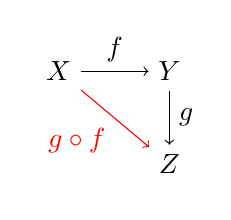
\begin{tikzpicture}[every node/.style={midway}]
\matrix[column sep={4em,between origins},
        row sep={2em}] at (0,0)
{ \node(A)   {$X$}  ; & \node(B) {$Y$}; \\
                      & \node(C) {$Z$}; \\};
\draw[->] (A) -- (B) node[anchor=south]  {$f$};
\draw[->] (B) -- (C) node[anchor=west]  {$g$};
\draw[->,red] (A) -- (C) node[anchor=north east] {$g\circ f$};
\end{tikzpicture}
\]
We do not really need to draw $g\circ f$ as a separate arrow because the \emph{path} from $X$ to $Y$ to $Z$ is already an implicit depiction of $g\circ f$.
So the simpler diagram 
\[
\tikzset{>=stealth}
\begin{tikzpicture}[every node/.style={midway}]
\matrix[column sep={4em,between origins},
        row sep={2em}] at (0,0)
{ \node(A)   {$X$}  ; & \node(B) {$Y$}; \\
                      & \node(C) {$Z$}; \\};
\draw[->] (A) -- (B) node[anchor=south]  {$f$};
\draw[->] (B) -- (C) node[anchor=west]  {$g$};
\end{tikzpicture}
\]
shows the same information, namely, that $\fromto fXY$ and $\fromto gYZ$ are functions and therefore, $\fromto {g\circ f}XZ$ is too.

Now a diagram such as this
\[
\tikzset{>=stealth}
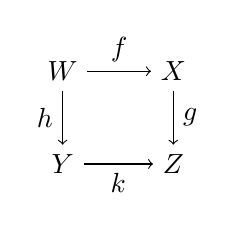
\begin{tikzpicture}[every node/.style={midway}]
\matrix[column sep={4em,between origins},
        row sep={2em}] at (0,0)
{ \node(A)   {$W$}  ; & \node(B) {$X$}; \\
  \node(D)   {$Y$}  ; & \node(C) {$Z$}; \\};
\draw[->] (A) -- (B) node[anchor=south]  {$f$};
\draw[->] (B) -- (C) node[anchor=west]  {$g$};
\draw[->] (A) -- (D) node[anchor=east] {$h$};
\draw[->] (D) -- (C) node[anchor=north] {$k$};
\end{tikzpicture}
\]
depicts two composite functions $g\circ f$ and $k\circ h$, but $g\circ f$ and $k\circ k$ may not be equal.
We say that the diagram \emph{commutes} or that it is a \emph{commutative diagram} if $g\circ f = k\circ h$.
In other words, saying that a certain diagram commutes \emph{is} an assertion that certain functions are equal.


\begin{exercises}
\begin{nextexercise}
\item  For each of the following pairs of functions $\NN\to\NN$, determine whether they are equal and explain why or why not.
  \begin{enumerate}
  \item $f(n) = 2n + 3$ and $g(m) = 2m + 3$
  \item $f(n) = 2^{n+1} - 1$ and $g(n) = \sum_{i=0}^n2^i$
  \item $f(n) =  n^2 + 5n + 6$ and $g(n) = (n+3)(n+2)$
  \item $f(n) = n^4 - 10n^3 + 35n^2 + 50n + 24$ and $g(n) = 24$
  \end{enumerate}
\item Let $\RR$ denote the set of all real numbers. Let $f(x) = \tan(x)$.
Explain why this does \emph{not} define a function from $\RR$ to $\RR$.
\item Suppose the following functions exist: $\fromto fWX$, $\fromto gXY$, $\fromto aWZ$, $\fromto bYZ$. 
  Draw a commutative diagram asserting that $b\circ g\circ f = a$.
\item Suppose the following functions exist: $\fromto fCA$, $\fromto gCB$, $\fromto hCP$, $\fromto pPA$ and $\fromto qPB$.
 Draw a commutative diagram asserting that $f=p\circ h$ and $g=q\circ h$.
\end{nextexercise}
\end{exercises}

\chapter{Constructing Sets and Functions}

\begin{goals}
	\noindent\textbf{Lecture}
	\begin{itemize}
	\item Characterize and define
		 \begin{itemize}
			 \item Pointer and constant functions
			\item Solution sets
			\item Characteristic functions
			%		 	\item The set of natural numbers
			\item Products of sets
			\item Exponents of sets
		 \end{itemize}
	\end{itemize}

	\noindent\textbf{Study}
	\begin{itemize}
	\item Be able to calculate membership in various constructed sets 
	\item Learn to use universal constructions to define functions. 
	\end{itemize}
\end{goals}

So far, we have thought mainly about informally defined sets and functions.
To fill out our understanding of sets, we need to be able to build sets and functions for specific purposes and with specific structure in mind. 

Three finite sets will play particularly important roles in this.
We have already discussed the set $\emptyset$, consisting of no elements.
We also need a designated set with one element and a designated set with two elements.
We denote these by $\One$ and $\Two$. 
It does not matter at all \emph{what} the elements are because, as we will soon see, sets of the same size are interchangable. 

For the time being, we merely need to agree on a fixed reference set with one element and a fixed reference set with two elements.
The particular choices we make here will be clearer as we put them to use.

\begin{defn}
	Let $\bullet$, $\bot$ and $\top$ be fixed symbols. Then define
	\begin{align*}
		\One &= \{\bullet\}\\
		\Two &= \{\bot,\top\}
	\end{align*} 
	The single element of $\One$ is intended to look like a generic point in an internal diagram.
	The element $\top$ is meant to remind you of the letter `T' (short for `True') and $\bot$ is meant to be the opposite of $\top$ ('False').
	These symbols are read as ``top'' and ``bottom''.
\end{defn}

%As mentioned above, the particular choice of elements is not important.
%Some folks would define $\One$ to be $\{0\}$ and $\Two$ to be $\{0,1\}$.
%This is convenient because the pattern continues: $\mathcal{3}$ would be $\{0,1,2\}$, and so on.
%We, however, wish to emphasize other things that have nothing directly to do with the numbers $0$ and $1$ (as members of $\One$ and $\Two$).

\section{Elements, Pointers and Constant Functions}

Suppose we are told that $\fromto p\One X$ is a function.
Since $\bullet\in\One$, this function determines an element of $X$, namely $p(\bullet)$.
A picture of the situation might be this:

\begin{figure}[h]
\[
  \begin{tikzpicture}[
    >=stealth,
    bullet/.style={
      fill=black,
      circle,
      minimum width=1pt,
      inner sep=1pt
    },
    projection/.style={
      ->,
      thick,
      shorten <=2pt,
      shorten >=2pt
    },
    every fit/.style={
      ellipse,
      draw,
      inner sep=0pt
    }
  ]
    \node[bullet] (p) at (0,2.5) {};

    \foreach \x/\y/\l in {4.1/1/4,3.2/2/3,4.3/3/2,4/4/1}
      \node[bullet,label=right:$\l$] (a\y) at (\x,\y) {};

    \node[draw,fit=(p),minimum width=1cm, minimum height=1cm] {} ;
    \node[draw,fit=(a1) (a2) (a3) (a4),minimum width=2cm] {} ;

    \draw[projection] (p) -- (a3);
  \end{tikzpicture}
\]
\caption{A function from $\One$ ``points'' to an element}\label{fig:pointer-example}
\end{figure}

Since $\bullet$ is the only element of $\One$, $p$ can ``point'' only to a single element of $X$.
So we might refer to a function $\sfromto p\One X$ as a \emph{pointer} into $X$.
Each pointer determines an element of $X$. 
And conversely, it should be possible to point to any element of $X$. 
This leads to a principle guaranteeing that certain (nearly trivial) functions exist.

\begin{principle}\label{ax:pointers}
	\noindent\textbf{Elements Determine Pointers}
	
	For any set $X$, and any $a\in X$, there is a function $\fromto {\hat a}\One X$ given by the rule $x\mapsto a$.
\end{principle}

Thus the function depicted in Figure \ref{fig:pointer-example} is $\hat{2}$. 
This principle simply asserts that elements of a set $X$ and functions $\One\to X$ are interchangible: from $a\in X$ we get $\fromto {\hat{a}}\One X$; from $\fromto p\One X$.
we get the element $p(\bullet)$.

Suppose $\fromto fX\One$ and $\fromto gX\One$ are functions, that is, their \emph{codomain} is $\One$ instead their \emph{domain}. 
Then $f(a)=\bullet = g(a)$ is true for every $a\in X$ because $\bullet$ is the only possible value. 
So $f=g$ by the Principle of Function Extensionality.
In other words, there is at most one function from $X$ to $\One$.
But the rule $x\mapsto \bullet$ is as simple a rule as one can imagine. 
This leads to another definition and another principle.

\begin{defn}\label{def:terminal}
	A set $T$ is \emph{terminal} if it is the case that for any set $X$ there is exactly one function from $X$ to $T$.
\end{defn}

\begin{principle}
	The set $\One$ is a terminal set. 
	We denote the unique function from $X$ to $\One$ by $\fromto {\Diamond_X}{X}\One$.
	
	The rule defining $\Diamond_X$ is
	\[x\mapsto\bullet.\]
\end{principle}

Using $\Diamond_X$ and $\hat{b}$ for an element $b\in Y$, we can now define a constant function. 
That is $\hat{b}\circ\Diamond_X$ is a function from $X$ to $Y$ given by the rule
$x\mapsto \hat{b}(\Diamond_X(x))= \hat{b}(\bullet) = b$. 
In short, this is the function sending all elements of $X$ to the constant $b$. 
It will be convenient to have a standard name for this function.

\begin{defn}
	For a sets $X$ and $Y$, and element $b\in Y$, let $\constant_{X,b} = \hat b\circ \Diamond X$. When $X$ is obvious form context, we omit it.
\end{defn}

\begin{exercises}
	\begin{firstexercise}
		\item Show that for any pointer $\fromto p\One X$, it is the case that $\widehat{p(\bullet)}=p$.
		\item Show that any set with exactly one element is a terminal set.
		\item Show that any terminal set has exactly one element.
		\item Suppose that $\fromto fXY$ is a function. Show that for every $a\in X$, $\widehat{f(a)} = f\circ \hat{a}$.
	\end{firstexercise}
\end{exercises}

\section{The Empty Set}

For trivial reasons, there is at most one function from $\emptyset$ to $X$,
for any set $X$. That is,  if $\fromto {f,g}\emptyset X$ are functions, then
for each $x\in\emptyset$, $f(x)=g(x)$ because there are no $x$'s to concern us. Hence by Principle \ref{ax:FunctionExtensionality}, $f=g$. The empty ``rule'' that tells us to do nothing specifies a function from $\emptyset$ to $X$. So for any set $X$, there is exactly one function from $\emptyset$ to $X$. Let's make that official.

\begin{defn}
	An \emph{initial set} is a set $I$ so that for any set $X$, there is exactly one function from $I$ to $X$.
\end{defn}

\begin{principle}
	The emptyset $\emptyset$ is an initial set. For a set $X$, the unique
	function from $\emptyset$ to $X$ (given by the empty rule) may be denoted by 
	$\fromto {\Box_A}\emptyset X$.
\end{principle}

Notice that a function $X\to\emptyset$ is impossible unless $X$ is also empty.
So $\emptyset$ is the only initial set. 

\begin{exercises}
	\begin{nextexercise}
		\item How many functions are there from $\emptyset$ to $\{a,b,c,d\}$? Explain.
		\item How many functions are there from $\{a,b,c,d\}$ to $emptyset$? Explain.
		\item How many functions are there from $\One$ to $\{a,b,c,d\}$? Explain.
		\item How many functions are there from $\{a,b,c,d\}$ to $\One$? Explain.
	\end{nextexercise}
\end{exercises}

\section{Solution Sets, Subsets, Characteristic Functions}

Suppose we are given two functions that are ``parallel'': $\fromto fXY$ and $\fromto gXY$. 
To aid readability, we will write this as $X\doublerightarrow{f}{g}Y$.
For some values $a\in X$, it might be the case that $f(a)=g(a)$.
Let us call such a value a \emph{particular solution to the equation $f(x)=g(x)$}. 

It might be the case that there are no particular solutions to an equation $f(x)=g(x)$.
For example, there are no natural numbers $n$ such that $n+1 = n$. 
On the other hand, there might be many particular solutions. 
For example, let $f(x)=x^3$ and let $g(x)= 6x^2 - 11x + 6$ both regarded as functions on the natural numbers.
Then it is easy to check that $1$, $2$ and $3$ solve the equation $f(x)=g(x)$.
In fact, these three are the only particular solutions.
We generalize as follows.

\begin{defn}\label{def:equalizer} 
	For two functions $X\doublerightarrow{f}{g} Y$, a \emph{solution} is a function $\sfromto sSX$ so that 
	$f\circ s = g\circ s$.
	Thus for example, if $a\in A$ is a particular solution then the pointer $\hat a$ is a solution.

	For functions $A\doublerightarrow{f}{g} B$, an \emph{equalizer} is a solution $\sfromto eEX$ so that for any solution $\sfromto sSX$, there is exactly one function $\sfromto hSE$ so that $e\circ h = k$.
\end{defn}

\begin{principle}
	For functions $X\doublerightarrow{f}{g} Y$, the collection of all particular solutions to the equation $f(x)=g(x)$ form a set, denoted by $\{x\in X\st f(x) = g(x)\}$. 	
	The function $\sfromto i{\{x\in X\st f(x)=g(x)\}}A$ given by the rule $x\mapsto x$ (called an \emph{inclusion map}) is an equalizer for $f$ and $g$.
	
	If $\sfromto sSX$ is a solution (that is, $f\circ s = g\circ s$),
	then the function $\sfromto {\check s}C{\{x\in A\st f(x)=g(x)\}}$ given by the rule 
	\[x\mapsto s(x)\]
	is the unique function for which $s = i\circ \check s$.
\end{principle}

This axiom tells us three main things.
First, we can form a subset of $X$ by specifying an equation $f(x)=g(x)$ for two functions $X\doublerightarrow{f}{g}Y$, and picking out the particular solutions.
Second, a subset formed in this way ``embeds'' in the given set $X$ by its inclusion map $i$.
Third, for any solution $s$, the function into the set of particular solutions is defined by the same rule as $s$.

External diagrams help us understand equalizers. 
An equalizer is a solution
\[
\begin{tikzpicture}
\matrix (m) [row sep=3em,column sep=4em,minimum width=2em]
{
	\node (E) {$E$}; & \node (A) {$X$}; & \node (B) {$Y$};\\
};
\draw[->, green] (E.east) -- node[anchor=north] {$e$} (A.west); 
\draw[->] (A.10) -- node[anchor=south]  {$f$} (B.170) ;
\draw[->] (A.350) -- node[anchor=north]  {$g$} (B.190);
\end{tikzpicture}
\]
so that if 
\[
\begin{tikzpicture}
\matrix (m) [row sep=3em,column sep=4em,minimum width=2em]
{
	\node (S) {$S$};\\
	\node (E) {$E$}; & \node (A) {$X$}; & \node (B) {$Y$};\\
};
\draw[->, red] (S.south east) -- node[anchor=south] {$s$} (A.north west);
\draw[->, blue] (E.east) -- node[anchor=north] {$e$} (A.west); 
\draw[->] (A.10) -- node[anchor=south]  {$f$} (B.170) ;
\draw[->] (A.350) -- node[anchor=north]  {$g$} (B.190);
\end{tikzpicture}
\]
is also a solution ($f\circ s=g\circ s$), then there is exactly one function making
\[
\begin{tikzpicture}
\matrix (m) [row sep=3em,column sep=4em,minimum width=2em]
{
	\node (S) {$S$};\\
	\node (E) {$E$}; & \node (A) {$X$}; & \node (B) {$Y$};\\
};
\draw[->,ForestGreen] (S.south) -- node[anchor=east] {$\check s$} (E.north);
\draw[->, red] (S.south east) -- node[anchor=south] {$s$} (A.north west);
\draw[->, blue] (E.east) -- node[anchor=north] {$e$} (A.west); 
\draw[->] (A.10) -- node[anchor=south]  {$f$} (B.170) ;
\draw[->] (A.350) -- node[anchor=north]  {$g$} (B.190);
\end{tikzpicture}
\]
commute.

\subsection*{Inverse Image of an Element}

Suppose $c\in Y$ and $\sfromto fXY$ is a function, then we can form the equalizer of $f$ and the constant function $\hat{c}\circ\Diamond_X$.
This is more easily written we $\{x\in X\st f(x)=c\}$.
Since it is common to pick out sets like this, special notation is in order.

\begin{defn}\label{def:inverse-image}
	For a function $\sfromto fXY$, and an element $c\in Y$, 
	\[f^-(c) = \{x\in X\st f(x)=c\}.\] 
	In this case, $f^-(c)$ is called the \emph{inverse image of $c$ with respect to $f$}.
\end{defn}

A diagram can help us understand inverse images as well. Suppose $\fromto fXY$ and $c\in C$,
then we can arrange a diagram 

\[
\begin{tikzpicture}
\matrix (m) [row sep=3em,column sep=4em,minimum width=2em]
{
	& \node (one) {$\One$};\\
	\node (A) {$X$}; & \node (C) {$Y$};\\
};
\draw[->] (A.east) -- node[anchor=north]  {$f$} (C.west) ;
\draw[->] (one.south) -- node[anchor=east]  {$\hat c$} (C.north);
\end{tikzpicture}
\]
The inverse image is a subset of $X$ with an inclusion map that makes the following diagram commute:
\[
\begin{tikzpicture}
\matrix (m) [row sep=3em,column sep=4em,minimum width=2em]
{
	\node (inv) {$f^-(c)$}; & \node (one) {$\One$};\\
	\node (A) {$A$}; & \node (C) {$C$};\\
};
\draw[->] (A.east) -- node[anchor=north]  {$f$} (C.west) ;
\draw[->] (one.south) -- node[anchor=west]  {$\hat c$} (C.north);
\draw[->,blue] (inv.south) -- node[anchor=east] {$i$} (A.north);
\draw[->,blue] (inv.east) -- node[anchor=south] {$\Diamond_{f^-(c)}$} (one.west);
\end{tikzpicture}
\]
For any other function $\sfromto gWX$ that makes following similar diagram commute:
\[
\begin{tikzpicture}
\matrix (m) [row sep=3em,column sep=4em,minimum width=2em]
{
	\node (B) {$W$};\\
	&\node (inv) {$f^-(c)$}; & \node (one) {$\One$};\\
	&\node (A) {$A$}; & \node (C) {$C$};\\
};
\draw[->] (A.east) -- node[anchor=north]  {$f$} (C.west) ;
\draw[->] (one.south) -- node[anchor=west]  {$\hat c$} (C.north);
\draw[->,blue] (inv.south) -- node[anchor=east] {$i$} (A.north);
\draw[->,blue] (inv.east) -- node[anchor=north] {$\Diamond_{f^-(c)}$} (one.west);
\draw[->,red] (B.south) -- node[anchor=east] {$g$} (A.north west);
\draw[->,red] (B.east) -- node[anchor=south] {$\Diamond_W$} (one.north west);
\end{tikzpicture}
\]
there is a unique function $\sfromto {\check g}B{f^-(c)}$ making
\[
\begin{tikzpicture}
\matrix (m) [row sep=3em,column sep=4em,minimum width=2em]
{
	\node (B) {$W$};\\
	&\node (inv) {$f^-(c)$}; & \node (one) {$\One$};\\
	&\node (A) {$X$}; & \node (C) {$Y$};\\
};
\draw[->] (A.east) -- node[anchor=north]  {$f$} (C.west) ;
\draw[->] (one.south) -- node[anchor=west]  {$\hat c$} (C.north);
\draw[->,blue] (inv.south) -- node[anchor=east] {$i$} (A.north);
\draw[->,blue] (inv.east) -- node[anchor=north] {$\Diamond_{f^-(c)}$} (one.west);
\draw[->,red] (B.south) -- node[anchor=east] {$g$} (A.north west);
\draw[->,red] (B.east) -- node[anchor=south] {$\Diamond_W$} (one.north west);
\draw[->, ForestGreen] (B.south east) -- node[anchor=west] {$\check g$} (inv.north west);
\end{tikzpicture}
\]
commute.

In Definition \ref{def:inverse-image}, the set $f^-(c)$ is a subset of $X$.
It would be good to know that any subset of $X$ can be described as an inverse image.
This is where the set $\Two$ plays a role.

\begin{defn}\label{def:subset-classifier}
	\noindent\textbf{Subset Classifier}
	
	A \emph{pointed set} is a set $P$ with a distinguished element $p\in P$.
	
	A \emph{subset classifier} is a set $T$ with a distinguished element $t\in T$ so that for any set $X$ and any subset $A\subseteq X$, there is exactly one function $\fromto kXT$ for which $A = k^-(t)$.
	That is, $A$ is uniquely defined as the inverse image of $t$ with respect to a function into $T$.
\end{defn}

\begin{principle}\label{ax:subset-char}
	\noindent\textbf{$\Two$ and Characteristic Functions}
	
	The set $\Two$ with the distinguished element $\top$ is a subset classifier.
	For subset $A\subseteq X$, the function corresponding to $A$, called the \emph{characteristic function of $A$}, is denoted by $\kappa_A$.
	In other words, $\kappa_A$ is the unique function for which $A = \kappa_A^-(\top)$.

	For $A\subseteq X$, the characteristic function is defined by the rule
	\[
	x \mapsto
		\begin{cases}
			\top &\text{if $x\in A$}\\
			\bot &\text{otherwise}
		\end{cases}
	\]
\end{principle}

Just as Principle \ref{ax:pointers} asserts that elements of $X$ and functions $\One\to X$ are interchangeable, Principle \ref{ax:subset-char} asserts that the subsets of $X$ and the functions $X\to\Two$ are interchangeable.

\begin{exercises}
	\begin{nextexercise}
	\item Draw a depiction of $A=\{a,b,c,d,e,f,g\}$ and its subset $B=\{a,c,e,g\}$ in the same internal diagram. Now depict the characteristic map for $B$ as a subset of $A$.
	
	\item Define two functions $\NN\doublerightarrow{f}{g}\NN$ so that the set of particular solutions of $f(x)=g(x)$ is $\{1,5\}$. 
	
	\item Consider the functions $\fromto f\RR\RR$ defined by $f(x) = \sin(x) + \cos(x)$, and $\fromto s\NN\RR$ defined by $s(n) = 2\pi n^2$. 
	Is $s$ a solution for the equation $f(x) = -1$? 
	What is the set of all particular solutions?
	
	\item Describe what a subset classifier is, using diagrams similar to the diagrams we have used to describe equalizers and inverse images.
	That is, for a start, we have a diagram
	\[
		\begin{tikzpicture}
	\matrix (m) [row sep=3em,column sep=4em,minimum width=2em]
	{
		\node (one) {$\One$};\\
		\node (S) {$T$};\\
	};
	\draw[->] (one.south) -- node[anchor=west]  {$\hat t$} (S.north);
	\end{tikzpicture}
	\]
	Now suppose we are given a subset $A\subseteq X$ with its inclusion map:
		\[
		\begin{tikzpicture}
		\matrix (m) [row sep=3em,column sep=4em,minimum width=2em]
		{
			\node (A) {$A$}; & \node (one) {$\One$};\\
			\node (X) {$X$}; & \node (S) {$S$};\\
		};
		\draw[->] (A.east) -- node[anchor=south] {$\Diamond_A$} (one.west);
		\draw[->] (A.south) -- node[anchor=east]  {$i$} (X.north);
		\draw[->] (one.south) -- node[anchor=west]  {$\hat t$} (S.north);
		\end{tikzpicture}
		\]
	What additional function is required to exist? What properties is it required to have? [Hint: the result should be that $A$ is an inverse image.]
	\end{nextexercise}
\end{exercises}

\section{Product Sets and Functions of Two Arguments}

We should be able to deal with functions of more than one argument, such as a function $f(x,y) = x^2+y^2$.
To account for these, we take our cue from Descartes.

Descartes studied the geometric plane in terms of a coordinate system consisting of the so-called $x$-axis and $y$-axis (what we call cartesian coordinates in his honor).
Once we have decided where to place the axes (as long as they do not run in parallel), a pair such as $(2,3)$ determines a point on the plane, and any point $p$ in the plane determines a pair.
So Descartes realized that we might as well just say that the plane actually \emph{is} the collection of all pairs of real numbers.
What makes this work is that points in the plane \emph{project} onto the two axes in a universal way.
Products of sets generalize this idea.

\begin{defn}
For sets $X$ and $Y$, a \emph{table} consists of two functions $X\stackrel{f}{\longleftarrow} T\stackrel{g}{\longrightarrow}Y$.
Note that the two functions have the same domain. We may call the two functions \emph{legs} of the table.

For sets $X$ and $Y$, a \emph{product of $X$ and $Y$} is a table $X\stackrel{p}{\longleftarrow} P\stackrel{q}{\longrightarrow}Y$ so that for any table $X\stackrel{f}{\longleftarrow} T\stackrel{g}{\longrightarrow}Y$ there is exactly one function $\sfromto hTP$ for which $f = p\circ h$ and $g= q\circ h$. 
For a product, the legs $p$ and $q$ are called the \emph{projections}.
\end{defn}

\begin{principle}\label{ax:products}
	For sets $X$ and $Y$, the collection of all pairs $(x,y)$ where $x\in X$ and $y\in Y$ is a set, denoted by $X\times Y$. 
	The functions $X\stackrel{\pi_0}{\longleftarrow}{X\times Y}\stackrel{\pi_1}{\longrightarrow}Y$ given by the rules $(x,y)\mapsto x$
	and $(x,y)\mapsto y$ are projections. For $X\stackrel{f}{\longleftarrow}{T}\stackrel{g}{\longrightarrow}Y$, the unique function required by
	the product may be denoted by $\langle f,g\rangle$.

	For $X\stackrel{f}{\longleftarrow}{T}\stackrel{g}{\longrightarrow}Y$, the function $\sfromto {\langle f,g\rangle}T{X\times Y}$ is given by the rule $t\mapsto(f(t),g(t))$.
\end{principle}

As with equalizers and inverse images, products can be described in terms of diagrams.

A product of $X$ and $Y$ is depicted as an external diagram
	\[
	\begin{tikzpicture}
	\matrix (m) [row sep=3em,column sep=4em,minimum width=2em]
	{
		\node (A) {$X$}; & \node (P) {$P$}; & \node (B) {$Y$};\\
	};
	\draw[->, blue] (P.west) -- node[anchor=north] {p} (A.east);
	\draw[->, blue] (P.east) -- node[anchor=north] {q} (B.west);
	\end{tikzpicture}
	\]
so that for any other table over $X$ and $Y$:
	\[
	\begin{tikzpicture}
	\matrix (m) [row sep=3em,column sep=4em,minimum width=2em]
	{
		&\node (C) {$T$};\\
		\node (A) {$X$}; & \node (P) {$P$}; & \node (B) {$Y$};\\
	};
	\draw[->,red] (C.south west) -- node[anchor=south east] {$f$} (A.north east);
	\draw[->,red] (C.south east) -- node[anchor=south west] {$g$} (B.north west);
	\draw[->,blue] (P.west) -- node[anchor=north] {$p$} (A.east);
	\draw[->,blue] (P.east) -- node[anchor=north] {$q$} (B.west);
	\end{tikzpicture},
	\]
there is a unique function making 
	\[
	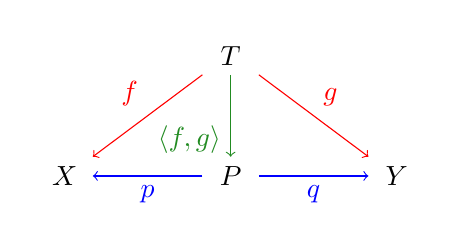
\begin{tikzpicture}
	\matrix (m) [row sep=3em,column sep=4em,minimum width=2em]
	{
		&\node (C) {$T$};\\
		\node (A) {$X$}; & \node (P) {$P$}; & \node (B) {$Y$};\\
	};
	\draw[->,ForestGreen] (C.south) -- node[anchor=north east] {$\langle f,g\rangle$} (P.north);
	\draw[->,red] (C.south west) -- node[anchor=south east] {$f$} (A.north east);
	\draw[->,red] (C.south east) -- node[anchor=south west] {$g$} (B.north west);
	\draw[->,blue] (P.west) -- node[anchor=north] {$p$} (A.east);
	\draw[->,blue] (P.east) -- node[anchor=north] {$q$} (B.west);
	\end{tikzpicture},
	\]
commute.		

Suppose we are given two unrelated functions $\sfromto fXY$ and $\sfromto gAB$. 
We can form a single function from $\sfromto{f\times g}{X\times A}{Y\times B}$ by combining $f$ and $g$ ``independently''. 
That is, define $f\times g = \langle f\circ \pi_0,g\circ \pi_1\rangle$.
Calculating concretely in terms of elements $(f\times g)(x,y) = (f(x),g(y))$. 
So $f\times g$ acts on a pair $(x,y)$ by applying $f$ to $x$ and unrelatedly applying $g$ to $y$.

Products can by generalized to three, four or more sets.
For example, given sets $X$, $Y$ and $Z$, we might write $X\times Y\times Z$ for the set of triples $(x,y,z)$ where $x\in X$, $y\in Y$ and $z\in Z$. 
Instead of two projections, this would have three projections $(x,y,z)\mapsto x$, and so on. 
It turns out, however, that binary products are enough because $X\times (Y\times Z)$ behaves just like $X\times Y\times Z$.

\begin{exercises}
	\begin{nextexercise}
		\item For the sets $A = \{a,b,c\}$ and $B = \{1,2,3,4\}$, write out $A\times B$ and $B\times A$
		\item What is $\emptyset \times A$? 
		\item Write out $\{4,a,0\}\times \Two$.
		\item Describe in plain English what are the elements of $\NN\times \NN$.
		\item Suppose $A$ is a finite set with $m$ elements and $B$ is a finite set with $n$ elements.
		How many elements are in $A\times B$?
		\item Describe in plain English why it makes sense to refer to $A\times B$ as a ``product.''
		\item For sets $A=\{a,b\}$, $B=\{0,1,2\}$ and $C=\{c,d\}$, calculate $A\times B\times C$, $A\times (B\times C)$ and $(A\times B)\times C$. Are these sets equal? If not, how do they differ.
		\item Describe a model of the standard fifty-two card poker deck as a product of two sets.
	\end{nextexercise}
\end{exercises}

\section{Function Sets and Parametric Functions}

A function from $X$ to $Y$ might depend on a parameter from another set $P$. 
For example, the function $\sfromto f\RR\RR$ given by the rule $x \mapsto \sin(x + c)$ depends on the constant $c$.
There is a related function $\sfromto g{\RR\times \RR}\RR$ given by $(c,x) \mapsto \sin(x+c)$.
Though $g$ describes the same behavior as $f$, it makes the parameter $c$ explicit as another argument. The relation between $f$ and $g$ leads to the following definition.

\begin{defn}
	For sets $P$, $X$ and $Y$, a \emph{parametric function from $X$ to $Y$} is a function $\sfromto g{P\times X}Y$ for some set $P$.
	The set $P$ will be called the \emph{parameter set}.
	
	Suppose $\sfromto f{Q\times X}Y$ is a parametric function with parameter set $Q$ and $\sfromto kPQ$ is a function.
	Then another parametric function with parameter set $P$ by composing: $f\circ (k\times \id_X)$.
	The function $k$ acts like a \emph{change of parameters} because it transforms the parametric function with parameters in $Q$ into a parametric function with parameters in $P$. 
	Specifically, $f\circ(k\times \id_X)$ is given by the rule $(c,a)\mapsto f(k(c),a)$.
	
	An \emph{evaluation map} for $X$ and $Y$ is a parametric function $\sfromto a{F\times X}Y$ with parameter set $F$, so that for any 
	parametric function $\sfromto g{P\times X}Y$ there is exactly one change of parameters $\fromto hPF$ so that
	$g = a\circ (h\times \id_X)$. In that case, $F$ is called an \emph{exponential with base $Y$ and exponent $X$}.
\end{defn}

\begin{principle}
	For sets $X$ and $Y$, the collection of all functions from $X$ to $Y$, denoted by $Y^X$, is a set.
	
	The rule $(f,x) \mapsto f(x)$ defines an evaluation map $\sfromto \appl{Y^X\times X}Y$.
	
	For a parametric function $\fromto f{P\times X}Y$, the unique function from $P$ to $Y^X$ determined by $f$ does not have a completely standard name.
	Increasingly, mathematicians honor the twentieth century logician, Haskell Curry, by referring to this as `currying'.
	For these lectures, we follow that tradition and write $\curry[f]$ for the unique function satisfying $f = \appl\circ (\curry[f] \times \id_X)$.
	
	Calculating how $\sfromto {\curry[f]}P{Y^X}$ must behave, we see that for any parameter $p\in P$, $\curry[f](p)\in Y^X$ is the function from $X$ to $Y$ given by the rule $x\mapsto f(p,x)$.
\end{principle}

\subsection*{$\lambda$ Notation}

In defining $\curry[f]$, we needed to describe certain elements of $Y^X$.
But elements of $Y^X$ are functions. And a function typically is described by a rule.
So it would be convnient to have a notation that permits us to describe the behavior of a function without giving the function a name. 
The logician Alonzo Church was interested in the fundamental idea of just what \emph{is} a function. He proposed a notation for describing functions, writing things like $\lambda x.x^2$ to describe the function that squares its input. 
The Greek letter $\lambda$ means nothing.  It is used only as a marker to introduce a function. 
The ``$\lambda$'' notation is widely adopted in computer science. Indeed, it appears even in languages such as Python.  
We could make the $\lambda$ notation formal (as did Church), but for our purposes informality is enough. We use this notation to describe elements of $Y^X$. Several examples will help to explain this. 

\begin{example}
	\begin{itemize}
	\item For $f\in Y^X$ and $g\in Z^Y$, the composite function $g\circ f\in Z^X$ is $\lambda x.g(f(x))$.
	
	\item The element of $\NN^\NN$ defined by $\lambda x.x^\nxt$ is the successor function.
	
	\item For any $a\in X$, the function $\hat a \in X^\One$ is $\lambda x.a$.
	
	\item For $X\stackrel{f}{\longleftarrow}T\stackrel{g}{\longrightarrow}Y$, the function
	${\langle f,g\rangle}{X\times Y}^T$ is $\lambda x.(f(x),g(x))$.
	
	\item For a parametric function $\sfromto f{P\times X}Y$, the function $\sfromto {\curry[f]}{P}{Y^X}$ can be defined by the rule $p\mapsto \lambda x.f(p,x)$.
	
	\item For any $f\in Y^X$, $f = \lambda x.f(x) = \lambda y.f(y)$. 

	\item The only element of $\One^X$ is $\lambda x.\bullet$.
	\end{itemize}
\end{example}
 
\begin{exercises}
	\begin{nextexercise}
		\item  For set $A= \{1,2,3\}$ and $B = \{a,b\}$ 
			\begin{enumerate}
				\item draw internal diagrams corresponding to each element of $B^A$ (there are eight of them);
				\item draw internal diagrams corresponding to each element of $A^B$ (there are nine of them).
			\end{enumerate}
		\item If $X$ is a finite set with $k$ elements, $Y$ is a finite set with $j$ elements, how many elements are there in the set $Y^X$? 
		\item Consider the function $\sfromto f{\NN\times\NN}\NN$ defined by
		      $f(m,n) = m^n$. What element of $\NN^\NN$ is $\curry[f](3)$? Use $\lambda$ notation to describe it.
		\item For the function $\min$ from $\RR\times\RR$ to $\RR$ defined to mean the minimum of $x$ and $y$, define $\curry[\min]$.
		\item Use $\lambda$ notation to describe the element of $\NN^\NN$ that quadruples the square of the input.
	\end{nextexercise}	
\end{exercises}

%\section{Universal Constructions}
%
%Consider the product $A\times B$ again.
%It possesses functions 
%$A\stackrel{\pi_0}{\longleftarrow}A\times B\stackrel{\pi_1}{\longrightarrow}B$. For any other similar arrangement
%$A\stackrel{f}{\longleftarrow}C\stackrel{g}{\longrightarrow}B$, there is a unique function $C\stackrel{\langle f,g\rangle}{\longrightarrow}{A\times B}$ making the diagram
%\[
%\tikzset{>=stealth}
%\begin{tikzpicture}[every node/.style={midway}]
%\matrix[column sep={4em,between origins},row sep={2em}] at (0,0)
%{ 					&	& \node(T) {$T$}; &	& \\
%	\\
%	\node(A)   {$A$}; &	& \node(P) {$P$}; &	& \node(B) {$B$}; \\};
%\draw[->] (T) -- (A) node[anchor=south east]  {$f$};
%\draw[->] (T) -- (B) node[anchor=south west]  {$g$};
%\draw[->] (T) -- (P) node[anchor=north east] {$\langle f,g \rangle$};
%\draw[->] (P) -- (A) node[anchor=north] {$\pi_0$};
%\draw[->] (P) -- (B) node[anchor=north] {$\pi_1$};
%\end{tikzpicture}
%\]
%commute.
%
%An equalizer ($\{x\in A\st f(x)=g(x)\}$), a terminal object ($\One$) and an exponential ($B^A$) are also characterized by some special functions so that any similarly arranged functions determine a unique function making a suitable diagram commute.
%Go back and reread the definitions of equalizers, terminal objects, products and exponentials to see that they all have this family resemblance.
%They are called \emph{universal constructions}.
%So the inclusion $\{x\in A\st f(x)=g(x)\}\to A$ is universal for solving the equation $f=g$; $A\stackrel{\pi_0}{\longleftarrow}A\times B\stackrel{\pi_1}{\longrightarrow}B$ is universal for mapping into $A$ and $B$;
%$B^A\times A\stackrel{\appl}B$ is the universal parametric function from $A$ to $B$.
%The principles of this lecture spell out that there are sets and functions 
%with the desired universal properties.
%
%\begin{exercises}
%	\begin{enumerate}
%		\item Explain how $\One\stackrel{\hat{\top}}{\longrightarrow}\Two$ is universal. [There is not a single intended correct answer to this. 
%		I want you to think about how $\Two$ fits into a bigger picture.]
%	\end{enumerate}
%\end{exercises}

\section{Embeddings and Quotients}

As we know, the fact that addition is cancellative ($m+p=n+p$ implies $m=n$) is quite useful. Likewise, multiplication is amost always cancellative ($m\cdot p=n\cdot p$ implies $m=n$ provided $p\neq 0$). And even list concatenation is cancellative. But function composition is not. At least not generally. It will turn out though that certain functions can indeed by cancelled on the left and others can be cancelled on the right. The role of these special functions is akin to the role that non-$0$'s play in multiplication.

\begin{defn}
	A function $\fromto fXY$ is called
	\begin{itemize}
		\item a \emph{monomorphism} if it is the case that for every $W\doublerightarrow{h}{k}X$, if $f\circ h=f\circ k$ then $h=k$;
		\item an \emph{epimorphism} if it is the case that 
		for every $Y\doublerightarrow{h}{k}Z$, if $h\circ f=k\circ f$ then $h=k$.
	\end{itemize}
\end{defn}

The terms \emph{mono-} and \emph{epi-} refer to behavior that we explore in this Lecture. For now, just commit them to memory: monomorphism \emph{cancel on the left} of $\circ$, epimorphisms \emph{cancel on the right}.

\begin{example}
	\begin{itemize}
	\item For any subset $A\subseteq X$, the inclusion function $\sfromto iAX$ is a monomorphism.
	\item  For sets $X$ and $Y$, the projection functions $\sfromto {\pi_0}{X\times Y}X$ and $\sfromto {\pi_1}{X\times Y}Y$ are epimorphisms.
	\item The functions $\sfromto {\Diamond_X}X\One$ are almost always epimorphisms. The only except is when $X=\emptyset$.
	\item All pointers $\sfromto {\hat a}{\One}X$ for $a\in X$ are monomorphisms.
	\item For any set $X$, $\id_X$ is both a monomorphism and an epimorphism.
	\end{itemize}
\end{example}

\begin{exercises}
	\begin{firstexercise}
		\item Show that if $\sfromto fXY$ and $\sfromto gYZ$ are epimorphisms, then so is $g\circ f$. 
		\item Show that if $\sfromto fXY$ and $\sfromto gYZ$ are monomorphisms, then so is $g\circ f$. 
	\end{firstexercise}
\end{exercises}

The definitions of mono- and epimorphisms refer to external behavior. The next two lemmas spell out equivalent internal behavior.

\begin{defn}
	A function $\sfromto fXY$ is called
	\begin{itemize}
		\item \emph{one-to-one} or \emph{injective} or \emph{an injection} if it is the case that for every $b\in Y$ there is at most one $a\in X$ so that $f(a)=b$;
		\item \emph{onto} or \emph{surjective} or \emph{a surjection} if it is the case that for every $b\in Y$ there is at least one $a\in X$ so that $f(a)=b$.
	\end{itemize}
\end{defn}

The property of being injective can also be stated by saying that if $f(a_0)=f(a_1)$ then $a_0=a_1$.

\begin{lemma}
	A function is a monomorphism if and only if it is an injection.
	
	\begin{proof}
		Assume $\sfromto mXY$ is a monomorphism. Consider $a_0,a_1\in X$ so that $m(a_0)=m(a_1)$.
		Then $m\circ \hat{a_0} = m\circ \hat{a_1}$. Since $m$ is a monomorphism $\hat{a_0} = \hat{a_1}$. Hence $a_0=a_1$.
		
		Assume $\sfromto mXY$ is not a monomorphism. 
		So there must be some set $W$ and functions $W\doublerightarrow{h}{k}X$ so that $m\circ h=m\circ k$ but $h\neq k$.
		Since $h\neq k$, there must be an element $w\in W$ so that $h(w)\neq k(w)$. 
		Let $a_0=h(w)$ and $a_1=k(w)$. 
		These witness that $m$ is not an injection because $m(a_0)=m(a_1)$ but $a_0\neq a_1$.
	\end{proof}
\end{lemma}

\begin{lemma}
	A function is an epimorphism if and only if it is a surjection.
	
	\begin{proof}
		Assume $\sfromto eXY$ is not onto. So there is some $b\in Y$ for which $e(x)\neq y$ is the case for all $x\in X$. Define $Y\doublerightarrow{h}{k}\{0,1,2\}$ by
		\begin{align*}h(y) &= \begin{cases}
			0 &\text{if $y=b$}\\
			2 &\text{otherwise}
			\end{cases}\\
			k(y) &= \begin{cases}
			1 & \text{if $y=b$}\\
			2 &\text{otherwise.}
			\end{cases}
		\end{align*}
		It is easy to verify that $h\circ e = k\circ e$, but obviosly $h\neq k$. So $e$ is not an epimorphism.
		
		Assume $\sfromto eXY$ is onto. Suppose $Y\doublerightarrow{h}{k}Z$ 
		satisfy $h\circ e=k\circ e$. For any $y\in Y$, there is some $x\in X$ so that $e(x)=y$. So $h(y)=h(e(x))=k(e(x))=k(y)$. By function extensionality, $h=k$.
	\end{proof}
\end{lemma}

Subsets permit us to concentrate attention on elements with special properties.
For an informal example, let $[-1,1]\subseteq\RR$ be the set of real numbers satisfying $-1\leq x\leq 1$.
Then the trigonometric function $\fromto \sin\RR\RR$ has the property that $\sin(x)\in [-1,1]$ is true for every $x\in\RR$.
So this suggests that $\sin$ can be ``co-restricted'' to the smaller codomain of $[-1,1]$. In fact, Principle \ref{ax:subset-char} guarantees this.
We need, however, to generalize the idea to situations not covered by the principle as stated.

Consider the two functions depicted in Figure \ref{fig:coinvariance-example}. Thhe function $m$ is a monomorphism. The two functions are related by having the same codomain. Moreover, the elements of the codomain that are reached by the function $f$ are also reached by $m$ ($f(x)=m(d)$, $f(y)=m(a)$ and $f(z)=m(a)$). So it makes sense to define a function as indicated in \ref{fig:factoring-through}. The situations in which this should be possible can be characterized internally via the behavior of functions on elements, or externally via their behavior with other functions. 

\begin{figure}
\[
  \begin{tikzpicture}[
  >=stealth,
  bullet/.style={
  	fill=black,
  	circle,
  	minimum width=1pt,
  	inner sep=1pt
  },
  projection/.style={
  	->,
  	thick,
  	shorten <=2pt,
  	shorten >=2pt
  },
  every fit/.style={
  	ellipse,
  	draw,
  	inner sep=0pt
  }
  ]
  \foreach \x/\y/\l in {0.4/1/a,-0.2/1.5/b,0/2/c,0.5/2.5/d}
  \node[bullet,label=left:$\l$] (a\l) at (\x,\y) {};
  
  \foreach \x/\y/\l in {4.1/3/0,4.6/2.5/1,5.2/2/2,5.7/1.5/3,6.1/1/4}
  \node[bullet,label=right:$\l$] (b\l) at (\x,\y) {};
  \node (brt) at (6.2,1) {};
  \node (blt) at (3.8,2) {};
  
  \foreach \x/\y/\l in {4.6/6/x,5.2/6.2/y,5.8/6.1/z}
  \node[bullet,label=right:$\l$] (c\l) at (\x,\y) {};
  \node (clo) at (5.2,5.7) {};
  \node (chi) at (5.2,6.3) {};
  
  \node[draw,fit=(aa) (ab) (ac) (ad),minimum width=2cm] {} ;
  \node[draw,fit=(b0) (b1) (b2) (b3) (b4) (brt) (blt), minimum width=2cm] {} ;
  \node[draw,fit=(cx) (cy) (cz) (clo) (chi), minimum width=2cm] {} ;
  
  \node at (2.5,.5) {$m$};
  \node at (6.3,3.8) {$f$};
  
  \draw[projection] (ad) -- (b1);
  \draw[projection] (ac) -- (b2);
  \draw[projection] (ab) -- (b3);
  \draw[projection] (aa) -- (b4);
  \draw[projection] (cx) -- (b1);
  \draw[projection] (cy) -- (b4);
  \draw[projection] (cz) -- (b4);
  
  \end{tikzpicture}
\]
	\caption{Function $f$ and $m$ with a common codomain}\label{fig:covariance-example}

\[
\begin{tikzpicture}[
>=stealth,
bullet/.style={
	fill=black,
	circle,
	minimum width=1pt,
	inner sep=1pt
},
projection/.style={
	->,
	thick,
	shorten <=2pt,
	shorten >=2pt
},
every fit/.style={
	ellipse,
	draw,
	inner sep=0pt
}
]
\foreach \x/\y/\l in {0.4/1/a,-0.2/1.5/b,0/2/c,0.5/2.5/d}
\node[bullet,label=left:$\l$] (a\l) at (\x,\y) {};

\foreach \x/\y/\l in {4.1/3/0,4.6/2.5/1,5.2/2/2,5.7/1.5/3,6.1/1/4}
\node[bullet,label=right:$\l$] (b\l) at (\x,\y) {};
\node (brt) at (6.2,1) {};
\node (blt) at (3.8,2) {};

\foreach \x/\y/\l in {4.6/6/x,5.2/6.2/y,5.8/6.1/z}
\node[bullet,label=right:$\l$] (c\l) at (\x,\y) {};
\node (clo) at (5.2,5.7) {};
\node (chi) at (5.2,6.3) {};

\node[draw,fit=(aa) (ab) (ac) (ad),minimum width=2cm] {} ;
\node[draw,fit=(b0) (b1) (b2) (b3) (b4) (brt) (blt), minimum width=2cm] {} ;
\node[draw,fit=(cx) (cy) (cz) (clo) (chi), minimum width=2cm] {} ;


\node at (2.5,.5) {$m$};
\node at (6.3,3.8) {$f$};
  

\draw[projection] (ad) -- (b1);
\draw[projection] (ac) -- (b2);
\draw[projection] (ab) -- (b3);
\draw[projection] (aa) -- (b4);
\draw[projection] (cx) -- (b1);
\draw[projection] (cy) -- (b4);
\draw[projection] (cz) -- (b4);
\draw[projection,blue] (cx) -- (ad);
\draw[projection,blue] (cy) -- (aa);
\draw[projection,blue] (cz) -- (aa);

\end{tikzpicture}
\]	
	\caption{Function $f$ \emph{factors uniquely through $m$}}\label{fig:factoring-through}
\end{figure}

Monomorphisms act like subsets, in the sense that if $A\subseteq X$, then the inclusion function $\sfromto iAX$ is a monomorphism. Our next principle stipulates that monomorphisms behave like subsets, also in the sense that they determine characteristic functions.

\begin{principle}
	For a monomorphism $\sfromto mXY$ there is a unique function $\sfromto {\kappa_m}Y\Two$ so that $m$ is an equalizer for the equation $\kappa_m(y) = \top$. 
	In other words, if $\sfromto fWY$ is a function satisfying $\kappa_m(f(w))=\top$ for all $w\in W$, then there is a unique function $\sfromto {m\backslash f}WX$ so that $f = (m\backslash f)\circ m$.  
	We say that $f$ \emph{factors through $m$ uniquely}.
	
	For a monomorphism $\sfromto mXY$, the characteristic function $\kappa_m$ is defined by
	\[\kappa_m(y) = \begin{cases}
	    \top & \text{if $y = m(x)$ for some $x\in X$}\\
	    \bot & \text{otherwise}.
	\end{cases}\]
	Suppose $\sfromto fWY$ is a function satisfying $\kappa_m(f(w)) = \top$ for all $w$. Then $(m\backslash f)(w) = x$ if and only if $f(w)=m(x)$. 
\end{principle}

In Figure \ref{fig:covariance-example}, the function $f$ satisfies $\kappa_m\circ f = \constant_\top$, so there is indeed a unique function $(m\backslash f)$ as indicated in Figure \ref{fig:factoring-through}.

To detect that $f$ is a solution of the equation $\kappa_m(y)=\top$ is a simple matter. An internal characterization is this: for every $w\in W$, there is some $x\in X$ so that $f(w)=m(x)$. An external characterization is also useful.

\begin{defn}
	For functions $X\stackrel{m}{\longrightarrow}Y\stackrel{f}{\longleftarrow}W$, say that $f$ is {$m$-coinvariant} if it is that case that for all $Y\doublerightarrow{h}{k}Z$, $h\circ m=k\circ m$ implies $k\circ f = h\circ f$.
\end{defn}

\begin{lemma}
	For function $X\stackrel{m}{\longrightarrow}Y\stackrel{f}{\longleftarrow}W$ where $m$ is a monomorphism, $f$ is $m$-coinvariant if and only if $\kappa_m\circ f = \constant_\top$.

\begin{proof}
	First, note that $\kappa_m\circ f = \constant_\top$ if and only if
	$\kappa_m(f(w))=\top$ for every $w\in W$. But $\kappa_m(y)=\top$ if and only if there is some $x\in X$ so that $y=m(x)$. Therefore, $\kappa_m\circ f=\top$ if and only if for every $w\in W$ there exists some $x\in X$ for which $f(w)=m(x)$.
	
	Assume $\kappa_m\circ f=\constant_\top$, and $h\circ m = k\circ m$. For any $w\in W$, there is some $x\in X$ so that $f(w)=m(x)$. Hence $h(f(w)) = h(m(x)) = k(m(x)) = k(f(w))$ for a suitable choice of $x$. 
	Since this works for any $w$, $h\circ f=k\circ f$. 
	
	Assume there is some $w\in W$ for which $f(w)\neq m(x)$ for all $x\in X$. Define functions $Y\doublerightarrow{h}{k}\{0,1,2\}$ by 
	\begin{align*}h(y) &= \begin{cases}
				0 &\text{if $y=f(w)$}\\
				2 &\text{otherwise}
	\end{cases}\\
	k(y) &= \begin{cases}
	1 & \text{if $y=f(w)$}\\
	2 &\text{otherwise.}
	\end{cases}
	\end{align*}
	It is easy to verify that $h\circ m = k\circ m$, but $h\circ f \neq k\circ k$. So $f$ is not $m$-coinvariant.
\end{proof}
\end{lemma}


\begin{lemma}\label{lem:coinvariant-factoring}
	For functions $W\stackrel{m}{\longrightarrow}Y\stackrel{f}{\longleftarrow}X$ where $m$ is an monomorphism and $f$ is $m$-coinvariant, there is a unique function $\sfromto {m\backslash f}XW$ so that $f = m\circ (m\backslash f)$.
	
	\begin{proof}
		There is nothing new to prove. Lemma \ref{lem} ensures that $\kappa_m\circ f = \constant_\top$. Principle \ref{princ:subobjects} ensures that $m\backslash f$ exists. 
	\end{proof}
\end{lemma}

Epimorphisms are dual to monomorphisms (they cancel on the left instead of on the right). The concept of $m$-coinvariance also has a useful dual.

\begin{defn}
	For functions $W\stackrel{f}{\longleftarrow}Y\stackrel{e}{\longrightarrow}X$, say that $f$ is {$e$-coinvariant} if it is that case that for all $Z\doublerightarrow{h}{k}Y$, $e\circ h=e\circ k$ implies $f\circ h = f\circ k$.
\end{defn}

\begin{lemma}\label{lem:invariant-factoring}
	For functions $W\stackrel{f}{\longleftarrow}Y\stackrel{e}{\longrightarrow}X$ where $e$ is an epimorphism and $f$ is $e$-invariant, there is a unique function $\sfromto {f/e}XW$ so that $f = (f/e)\circ e$.
	
	\begin{proof}
		A full proof is technical and not especially informative. 
		The idea is that $f/e$ can be defined by a ``rule'': $e(y) \mapsto f(y)$. 
		Obviously, this does not look like a rule sending elements of $X$ to elements of $W$, but in fact it is. 
		This is because each $x\in X$ takes the form $e(y)$ for some $y$ because $e$ is onto. 
		And because $f$ is $e$-invariant, the choice of $y$ so that $e(y)=x$ does not matter for the resulting value $f(y)$.
		So the rule does indeed pick a single value $(f/e)(x)$ for each $x\in X$.  
	\end{proof}
\end{lemma}

Comparing Lemmas \ref{lem:coinvariant-factoring} and \ref{lem:invariant-factoring}, we note that monomorphisms are equalizers, so they behave in most respects like subsets. So a question arises as to what should be the analogue of an epimorphism. That is, what things built from elements of a set $X$ correspond to epimorphisms in analogy with the way subsets correspond to monomorphisms.

\begin{defn}
	For a set $X$, a \emph{partition on of $X$} is a subset $P\subseteq \powerset(X)$ so that
	\begin{itemize}
		\item for each $B\in P$, there is an $x\in X$ so that $x\in B$; and 
		\item for each $x\in X$, there is a $B\in P$ so that $x\in B$.
	\end{itemize}
\end{defn}

\chapter{The Set of Natural Numbers}\label{lec:natural-numbers}

\begin{goals}
\noindent\textbf{Lecture:}
\begin{itemize}
	\item Re-introduce the natural numbers as a set
	\item Introduce sequences and recursively defined sequences
	\item Relate recursion to proofs by induction
\end{itemize}

\noindent\textbf{Study:}
\begin{itemize}
	\item Be able to define simple functions by recursion
	\item Be able to explain how induction and recursion are related
\end{itemize}
\end{goals}

We have used $\NN$ informally to denote the set of natural numbers. 
It is time that we make the structure of $\NN$ explicit within our theory of sets and functions. 
It will turn out that $\NN$ is also a universal construction. 

Natural numbers provide a precise picture of counting and of putting things in an order.
Now that we have sets and functions we can consider a function $\fromto a\NN A$ to be an \emph{infinite sequence}: $a(0)$, $a(1)$, $a(2)$, \ldots.
When we do that, we sometimes write $a_0$, $a_1$, $a_2$, \ldots instead.
Still $a$ itself is just function from $\NN$ to $A$.
To emphasize the notation that $a$ represents an infinite sequence, we sometimes also write $(a_i)_{i\in I}$.

Much of what we discuss in this lecture has the feel of computer programming.
This is partly because natural numbers are the main objects of calculation.
We want to understand, for example, how to define a function like $n\mapsto n!$ ($n$ factorial) as a function from $\NN$ to $\NN$ by specifying how it is calculated.
In particular, $0! = 1$ and $(n^\nxt)! = n^\nxt\cdot n!$ characterize factorial by spelling out how to calculate it.
For example,
\begin{align*}
	4!  &= 4 \cdot 3! \\
		&= 4 \cdot (3 \cdot 2!)\\
		&= 4 \cdot (3 \cdot (2 \cdot 1!))\\
		&= 4 \cdot (3 \cdot (2 \cdot (1 \cdot 0!)))\\
		&= 4 \cdot (3 \cdot (2 \cdot (1 \cdot 1)))
		&= 24
\end{align*}

It is quite common to think about a sequence in which $a_{n+1}$ is functionally related to $a_n$. 
For example, in the sequence $1, 2, 4, 8,\ldots$, the initial entry is $1$ and each successive entry is double its predecessor.

Indeed, if we know just those two facts -- the initial entry is $1$, and each subsequent entry is double its predecessor -- then we know how the entire sequence behaves.
Also, we know how to calculate the $n^{\text{th}}$ entry, by recursion just like factorial.

The most basic sequence, of course, is $0$, $1$, $2$, \ldots. 
Its initial entry is $0$ and each subsequent entry is the successor of its predecessor. 
So we think of the sequence that comprises $\NN$ as a universal recursively defined sequence.

\section{Sequences and Simple Recurrences}

Let us make the informal word \emph{sequence} official.

\begin{defn}
	A \emph{sequence in set $X$} is a function $\fromto a\NN X$.
\end{defn}

As we studied in previous lectures, the basic vocabulary of natural numbers is that (i) there is a starting natural number, $0$, and (ii) for each natural number $n$ there is a next one, $n^\nxt$. 
To discuss successor in the language of sets and functions, we stipulate that successor is a function $\fromto \suc\NN\NN$ given by the rule $n\mapsto n^\nxt$.
So $\NN$ is not just a set. 
It comes with functions $\One \stackrel{\hat{0}}{\longrightarrow} \NN \stackrel{\suc}{\longleftarrow} \NN$.

Suppose $\One\stackrel{\hat{b}}{\longrightarrow}X\stackrel{r}{\longleftarrow}X$ is a similar structure.
Then we ought to be able to define a $a$ sequence in $X$, so that $a_0=b$, $a_1=r(b)$, $a_2=r(r(b))$, and so on. 
In general, $a_k$ should be determined by starting with $b$ and repeatedly applying $r$ a total of $k$ times. 

\begin{defn}\label{def:nno}
	A \emph{simple recurrence} is a set with functions $\One\stackrel{\hat{b}}{\longrightarrow}X\stackrel{r}{\longleftarrow}X$. We will say the two functions $\hat{b}$ and $r$ form a \emph{recurrence on $X$}.
	
	A \emph{natural number set} is a simple recurrence   $\One\stackrel{\hat{z}}{\longrightarrow}N\stackrel{s}{\longleftarrow}N$ so that for any other simple recurrence $\One\stackrel{\hat{b}}{\longrightarrow}X\stackrel{r}{\longleftarrow}X$, there is exactly one function $\sfromto fNX$ so that $f\circ \hat{z} =\hat b$ and $f\circ s = r\circ f$.
\end{defn}

The principle we are interested in here is that simple recurrences determine sequences.

\begin{principle}\label{ax:nat-numbers}
	The collection of natural numbers is a set, denoted by $\NN$.
	Moreover, $\One \stackrel{\hat{0}}{\longrightarrow} \NN \stackrel{\suc}{\longleftarrow} \NN$.
	makes $\NN$ a natural numbers set.
	
	From a simple recurrence $\One \stackrel{\hat{b}}{\longrightarrow} X \stackrel{r}{\longleftarrow} X$, the corresponding unique sequence in $X$
	may be denoted by $\srec[b,r]$. So $\sfromto {\srec[b,r]}\NN X$ is characterized by
	\begin{align*}
		\srec[b,r]_0 &= b\\
		\srec[b,r]_{n^\nxt} &= r(\srec[b,r]_n)
	\end{align*}
\end{principle}

So every simple recurrence on a set $X$ determines a sequence in $X$. 
On the other hand, it is not the case that every sequence is determined by a simple recurrence.
Take for example, the sequence $0,1,0,2,0,3,\ldots$. 
This can not be defined (at least not directly) by giving an initial entry and specifying successive entries based only on the predecessors. 
After all, the entries $1$, $2$, $3$ and so on all have the same preceding entry.


\section{Primitive Recursion}

Evidently, addition, multiplication, factorial, and other familiar functions should be definable using Principle \ref{ax:nat-numbers}. 
But there are problems to overcome: Addition is not a sequence, at least not in an obvious way. And factorial is not obviously definable by a simple recurrence
because we would need a function $\fromto r\NN\NN$ so that $n^\nxt! = r(n!)$
for all $n$. If, in place of $r$, we could use a function that depends on $n$ as well as on $n!$, we could define factorial recursively the usual way.

Putting things together, we consider a scheme that generalizes simple recursion to permit (i) dependence on a parameter not directly involved in the recursion, and
(ii) dependence on $n$ at each stage of the recursion.

\begin{defn}
	A \emph{primitive recurrence in $A$ (with parameters in $C$)} consists of two  functions $C\stackrel{b}{\longrightarrow} A\stackrel{r}{\longleftarrow}\NN\times C\times A$.
	
	A \emph{parametric sequence in $A$ with parameters in $C$} is a function
	$\fromto a{C\times \NN}A$. For a parametric sequence, we may write $a_{c,n}$
	instead of $a(c,n)$. 
\end{defn}

\begin{theorem}
	For any primitive recurrence $C \stackrel{b}{\longrightarrow} A \stackrel{r}{\longleftarrow} C\times \NN \times A$, there is a unique
	function $\fromto {\primrec[b,r]}{C\times \NN}A$ satisfying: 
	\begin{align*}
		\primrec[b,r]_{c,0} &= b(c)\\
		\primrec[b,r]_{c,k^\nxt} &= r(c,k,\primrec[b,r]_{c,k})
	\end{align*}

	\begin{proof}
		The proof of this requires additional ideas that are implict in the way subset classification (using $\Two$) works. We have all the principles we need, but a proof now would involve quite a long development. So we only sketch the rough idea.
		
		We use simple recursion to define a sequence of ``approximations'' of the desired function. First, let $D_n = C\times \{0,\dotsc,n\}$ for each $n\in\NN$. Then define 
		$\fromto {f_n}{D_n}A$ for each $n\in \NN$ by
		\begin{align*}
			f_0(c,0) &= b(c)\\
			f_{k^\nxt}(c,i) &= f_k(c,i) & \text{if $i\leq k$}\\
			f_{k^\nxt}(c,k^\nxt) = 	r(c,k,f_k(c,k)) & \text{otherwise}.
		\end{align*}
		Then define $\fromto f{C\times \NN}A$ by $f(c,n) = f_n(c,n)$. 
		It can be checked that $f$ satisfies the desired equations, and that no other function does.
		
		The technical part of the proof is mainly concerned with ensuring that the sequence of functions $f_n$ is indeed definable and that $f$ can be defined from those.  
	\end{proof}
\end{theorem}

\begin{example}
	The ``predecessor'' function is defined by the scheme $\pred(0)=0$ and $\pred(n^\nxt) = n$. 
	The primitive recurrence
	$\One \stackrel{\hat0}{\longrightarrow} \NN \stackrel{\pi_1}{\longleftarrow} \One\times\NN\times\NN$ where $\pi_1$ is the projection $(x,y,z)\mapsto y$ determines a function $\fromto g{\One\times \NN}{\NN}$ given by
	$g(\bullet, 0) = 0$ and $g(\bullet,n^\nxt) = \pi_2(\bullet, n, g(\bullet, n)) = n$. Hence, we may define $\pred(n) = g(\bullet, n)$
\end{example}

\begin{exercises}
\begin{firstexercise}
	\item Define addition $\sfromto {+}{\NN\times \NN}\NN$ by primitive recursion. That is, find functions $\sfromto b\NN\NN$ and $\sfromto r{\NN\times\NN\times \NN}\NN$ so that
	\begin{align*}
		m+0 &= b(m)\\
		m+n^\nxt &= r(m,n,m+n)
	\end{align*}
	That way, $\primrec[b,r]$ is addition.
	\item Define multiplication $\sfromto {\cdot}{\NN\times \NN}\NN$ by primitive recursion. You may use addition in defining the primitive recurrence.
	\item Define the factorial function by primitive recursion. You may use multiplication in defining the primitive recurrence.	
	\item For a given function $\fromto f\NN\NN$, find a primitive recurrence that defines the function $n\mapsto \sum_{i=0}^{n-1}f(i)$. That is, result will be the sequence $0$, $f(0)$, $f(0)+f(1)$, $f(0)+f(1)+f(2)$, \ldots.
	\item The operation of \emph{monus} $m\stackrel{.}{-} n$ is defined to be $m-n$ when $m \geq n$ and to be $0$ otherwise. Define monus by primitive recursion.
	\item Let $\sfromto p\NN\Two$ be a characteristic function. Show that bounded existential quantification is primitive recursive. That is, define the function $\fromto {\exists^<_p}\NN\Two$ by $\exists^p_<(n) = \top$ iff there is at least one $k<n$ for which $p(k)=\top$.  Show that this can be defined by a primitive recurrence.
	[Hint: $\exists^p_<(0) = \bot$ because there are no natural numbers below $0$. 
	Now ask what value is $\exists^p_<(n^\nxt)$ in terms of $p$ and $\exists^p_<(n)$.]
\end{firstexercise}
\end{exercises}

\section{Primitive Recursion and ``for'' loops}

It is a theorem (we will not prove here) that there is a technical sense in which primitive recursive functions exactly the functions  implementable, say in Python, by nested ``for'' loops. To get a taste of what this means, let us pretend that $\sfromto bPX$ and $\sfromto r{P\times \NN\times X}X$ are somehow defined by Python functions. Then the following code implements $\primrec[b,r]$.

\begin{lstlisting}
	def p_rec($b\in X^P$,$r\in X^{P\times \NN\times X}$) $\in X^{P\times \NN}$
		def $f$($p\in P$,$n\in \NN$): $\in X$
			$x = b(p)$
			for $i$ in range($n$):
				$x = r(p,i,x)$
			return $x$
		return $f$
\end{lstlisting}

Conversely, suppose a function in Python is defined using only natural number variables and the following parts of Python:
\begin{itemize}
	\item Assignment statements
	\item Increment statements: ``\lstinline!n+=1!''
	\item loops of the form ``\lstinline!for i in range(n): !\ldots''
	\item evaluations of functions that are defined similarly
\end{itemize}
The theorem we allude to claims that such a function is definable by primitive recursion. The theorem is not especially difficult, but it does involve a lot of careful checking. The point is that primitive recursion allows us to define a lot of the functions that we expect to be able to program in a standard programming language.

A question arises, however. If ``for'' loops are sufficient to program any primitive recursive function, why bother with other more complicated loops?
One answer is that programming languages are not merely for computing functions. They are used to implement lots of behavior that is not so easily cast in terms of sets and functions. Another answer, though, is internal to set theory. Namely, there are computable functions on $\NN$ which are not primitive recursive.

For each $n\in \NN$, define the sets $P^n\subseteq \NN^{\NN^n}$ of \emph{$n$-ary number theoretic primitive recursive functions} to be the smallest sets satisfying:
\begin{itemize}
	\item $\hat{0} \in P^0$
	\item $\suc\in P^1$
	\item for each $k<n$, $\pi^n_k\in P^n$ where $\pi^n_k\in \NN^{\NN^n}$ is defined by $\pi^n_k(x_0,\dotsc, x_{n-1}) = x_k$
	\item If $g\in P^n$ and for each $k<n$, $f_k\in P^m$, then $g\circ \langle f_0,\dotsc, f_{n-1}\rangle \in P^m$
	\item if $b\in P^m$ and $h\in P^{m+2}$, then $\primrec[b,h]\in P^{m+1}$
\end{itemize}

Consider the following sequence $A_0, A_1, \dotsc$ in ${\NN}^\NN$ defined by
\begin{align*}
A_0 & \suc\\
A_{k^\nxt} = \primrec[\hat{A_k(1)}, A_k\circ \pi^2_1]
\end{align*}
Putting this in terms of elements
\begin{align*}
	A_0(m) &= m+1\\
	A_{k^\nxt}(0) &= A_k(1)\\
	A_{k^\nxt}(m^\nxt) &= A_k(A_{k^\nxt}(m)).
\end{align*}
Evidently, each individual function $A_k$ is a number theoretic primitive recursive unary function. But
the function $\fromto {\symb{Ack}}\NN\NN$ defined by $\symb{Ack}(n) = A_n(n)$ is not. The proof is quite ingeneous. Roughly, one shows that $\symb{Ack}$ grows faster than any number theoretic primitive recursive function.

To get an idea of how fast this function grows, $\symb{Ack}(0) = 1$, $\symb{Ack}(1) = 3$, $\symb{Ack}(3) = 61$, $\symb{Ack}(4) = 2^{2^{65536}}-3$ a number vastly larger than the number of electrons in the visible universe. 
 
\section{Lists}

For a set $X$, the lists consisting of elements from $X$ also form a set.
The structure of this set is similar to $\NN$.

\begin{defn}
	For a set $X$, a \emph{simple $X$-recurrrence} is a set with two functions
	$\One \stackrel{\hat b}{\longrightarrow} A \stackrel{r}{\longleftarrow} X\times A$.
	
	For a set $X$, an \emph{$X$-list set} is a simple $X$-recurrence 
	$\One \stackrel{\hat{e}}{\longrightarrow} L \stackrel{c}{\longleftarrow} X\times L$ so that for any simple $A$-recurrence $\One \stackrel{\hat b}{\longrightarrow} A \stackrel{r}{\longleftarrow} X\times A$ there is exactly one function $\fromto hLA$ so that 
	\begin{align*}
		h\circ \hat e 	&= \hat b\\
		h\circ c 		&= r\circ (\id_X\times h).
	\end{align*}
\end{defn}

\begin{principle}
	The collection of lists with items drawn from $X$ is a set, denoted by $\List[X]$.
	The functions $\One\stackrel{\widehat{[\,]}}{\longrightarrow}\List[X]\stackrel{\mathord{:}}{\longleftarrow}X\times \List[X]$
	constitute an $X$-list set, where the function $\sfromto {\mathord{\colon}}{X\times \List[X]}{\List[X]}$ is the function given by the rule $(x,L)\mapsto x:L$.
	
	For $\One \stackrel{\hat b}{\longrightarrow} A \stackrel{r}{\longleftarrow} X\times A$, we reuse our notation for simle recursive functions on $\NN$
	and write $\srec[\hat b,r]$ for the unique function 
	satisfying 
	\begin{align*} 
	 \srec[\hat b,r]([\,]) &= b\\
	 \srec[\hat b,r](x:L)  &= r(x, \srec[\hat b, r](L))
	\end{align*}
\end{principle}

\begin{example}
	$\One \stackrel{\hat 0}{\longrightarrow} \NN \stackrel{+}{\longleftarrow} \NN\times \NN$ determine a function $\srec[\hat 0, +]$ from $\List(\NN)$ to $\NN$. The function satifies $\srec[\hat 0,+]([\,])= 0$ and $\srec[\hat 0,+](n:L)= n + \srec[\hat 0,+](L)$.
	So $\srec[0,+]$ returns the sum of items in a list natural numbers.
	Earlier, we wrote this as $\sum L$. In other words, we \emph{defined} $\mathord{\Sigma} = \srec[\hat 0,+]$.
\end{example}

Like $\NN$, $\List[A]$ supports a form of primitive recursion. 
The details can be worked out by the reader. 

\begin{exercises}
	\begin{nextexercise}
		\item For a function $\fromto fXY$, specify a simple $X$- recurrence that defines the function
			\[\fromto {\map[f]}{\List[X]}{\List[Y]}\] so that \[\map[f]([a_0,a_1,\ldots, a_{n-1}]) = [f(a_0),f(a_1),\ldots, f(a_{n-1})]\]
		\item For $\map[\cdot]$ as defined in the previous exercise, show that for any $\fromto fXY$ and $\fromto gYZ$, $\map[g\circ f] = \map[g]\circ \map[f]$.
		\item Define concatenation in $\List[A]$ by a simple $A$ recurrence. [Hint: I am asking for a function from $\List[A]\times \List[A]$ to $\List[A]$, but simple $A$ recurrence alone will not do the job, because that can only define a function $\List[A]\to X$ for some  $X$. Do this instead: (i) specify a simple $A$-recurrence to define a function $\fromto c{\List[A]}{\List[A]^{\List[A]}}$ for which $c(M)(L)$ is the concatetation of $L$ followed by $M$, (ii) define $L\star M$ to be $c(M)(L)$.
		\item Show that $\NN$ constitutes a $\One$-list set. That is, 
		describe two functions $\One\stackrel{\hat{e}}{\longrightarrow}\NN\stackrel{c}{\longleftarrow}\One\times \NN$ so that for any two functions $\One\stackrel{\hat{b}}{\longrightarrow}A\stackrel{r}{\longleftarrow}\One\times A$ there is a unique function $\sfromto f\NN A$
		satisfying
		\begin{align*}
			f(e) &= b\\
			f(c(x,y)) &= s(x,f(y)) 
		\end{align*}
		\item Write a scheme for ``primitive $X$-recursion'', specified by functions $P\stackrel{b}{\longrightarrow}A\stackrel{r}{\longleftarrow}P\times \List[X]\times A$. Write the equations involving $b$ and $r$ that should determine a unique function $P\times \List[X]\to A$. 
		You do not need to prove that your scheme actually defines a function.
	\end{nextexercise}
\end{exercises}

\chapter{Powersets}

\begin{goals}
	
\end{goals}

The exponential $\Two^X$ for a set $X$ is the set of all characteristic maps on $X$.
Each $k\in \Two^X$ corresponds to a subset of $X$ by $k^{-1}(\top) = \{x\in X\st k(x)=\top\}$. Vice versa, a subset $A\subseteq X$ determines a characteristic function $\fromto {\kappa_A}X\Two$ by the rule
\[x\mapsto \begin{cases}
			\top &\text{if $x\in A$}\\
			\bot &\text{otherwise}
\end{cases}
\]
So $\Two^X$ is, in this sense, \emph{representative} of the collection of all subsets of $X$. 
It is convenient also to suppose that the actual collection of subsets of a set $X$ forms a set.
This should ``behave'' exactly like $\Two^X$, but concretely, consist of subsets rather than characteristic functions.

\begin{principle}\label{ax:powerset}
	For any set $X$, the collection of subsets of $X$ is a set, denoted by $\powerset(X)$ and called the \emph{power set of $X$}. 
	Moreover, there is a function $\fromto {\ni_X}{\powerset(X)\times X}\Two$ defined by
	\[{\mathord\ni}_X(A,x) = \begin{cases}
	\top, &\text{ if } x\in A\\
	\bot &\text{otherwise}
	\end{cases}
	\]
	The function $\ni_X$ is an evaluation map, meaning that 
	for any function $\fromto f{P\times X}\Two$, there is a unique function $\fromto {f^\dagger}P{\powerset(X)}$ for which $f = {\mathord\ni}_X\circ (f^\dagger \times \id_X)$. The function $f^\dagger$ 
	is given by the rule $p\mapsto \{x\in X\st f(p,x)=\top\}$.
\end{principle}

For a function $\fromto fXY$, ${\mathord\ni}_Y\circ (\id_{\powerset(X)}\times f)$ is a function from $\powerset(Y)\times X$ to $\Two$. So there is a unique function
from $\powerset(Y)$ to $\powerset(X)$ determined by $f$ according to the above princple.
This is called \emph{inverse image}.

\begin{defn}
	For $\sfromto fXY$, let $\sfromto {f^-}{\powerset(Y)}{\powerset(X)}$ denote
	the unique function for which ${\mathord\ni}_B\circ (\id_{\powerset(B)}\times f) = {\mathord\ni}_A\circ(f^-\times \id_A)$. In terms of elements, $f^-$ satsifies
	\[x\in f^-(B) \text{if and only if } f(x)\in B\]
	for every $B\subseteq Y$.  So $f^-$ is given by the rule $B\mapsto \{x\in X\st f(x)\in B\}$
\end{defn}

This notation clashes slightly with our earlier definition of inverse image of an element, $f^-(b) = \{x\in X\st f(x)=b\}$. But this is harmless because 
$f^-(b)$ in the earlier usage is the same as $f^-(\{b\})$ in the new usage.

\begin{exercises}
	\begin{firstexercise}
		\item For $\fromto f\NN\NN$ defined by $f(n) = x^2$, what is $f^-(\{2,3,4,5,6,7,8\})$?
		\item For $\fromto \sin\RR\RR$, what is $\sin^-(\{-1,1\})$?
		\item Show that for any two functions $\fromto fXY$ and $\fromto gYZ$, $(g\circ f)^- = f^-\circ g^-$.
	\end{firstexercise}
\end{exercises}

\section{Finitary Structure of $\powerset(U)$}

Suppose we are currently interested in a particular set, which we will consider to be the ``universe of discourse.'' For example, for now we might only be interested in natural numbers. So our universe of discourse is $\NN$. Or we might be interested in poker. So our universe of discourse is $\symb{Deck}$, the set we defined earlier in these lectures. For this discussion, let us refer to this set as $U$ (for ``universe''). Then the structure of $\powerset(U)$ is of particular interest.

Suppose $A$ and $B$ are subsets of $U$. 
Then it makes sense to consider the elements that $A$ and $B$ have in common. 
For example, for $A\subseteq \NN$ being the set of even natural numbers and $B\subseteq \NN$ the set of perfect squares, we might want to concentrate on the set of even, perfect squares, which is another subset of $\NN$.
In general, for $A\subseteq U$ and $B\subseteq U$, the elements in common constitute another subset of $U$.
This is called the \emph{intersection} and is denoted by $A\cap B$.

Likewise, we might consider merging $A$ and $B$ into a single set (in our example, the set of numbers that are either even or perfect squares).
This is called the \emph{union}.
Related to intersection, there is a largest set $C$ so that $C\cap A\subseteq B$. 
This is called the \emph{residual}, and is denoted by $A\Rightarrow B$.
Flipping things the other way, there is also a smallest set $C$ so that $A\subseteq B\cup C$. This is called the \emph{set difference} and is denoted by $A\setminus B$. 

These operations on subsets of $U$ are closely related to the logic of propositions.
Imagine that $U$ consists of a ``universe'' of possible worlds. Then subsets of $U$ are collections of worlds where certain things are true.
For example, perhaps $P\subseteq U$ is the set of worlds in which pigs fly;
$K\subseteq X$ is the set of worlds in which kittens smoke cigars.
So $P\cap K$ is the set of worlds in which pigs fly \emph{and} kittens smoke cigars.
Likewise, $P\cup K$ is the set of worlds in which \emph{Either} pigs fly \emph{or} kittens smoke cigars.
And $P\Rightarrow K$ is the set of worlds in which it is true that if pigs fly, \emph{then} kittens smoke cigars. 

Understanding the interaction of $\cap$, $\cup$ and $\Rightarrow$ is closely related to the logic of ``and'', ``or'' and ``implies''. If we add a sentence ``False'' that is never true and another one ``True'' that is always true, then the logic of ``and'', ``or'' and ``implies'' form what is called a \emph{Heyting algebra}.

In fact, ``implies'' interacts with ``False'' in a useful way.
It turns out that ``$P$ implies False'' is essentially the same as saying ``$P$ is not true''. And if ``$P$ is not true'' is not true, then ``$P$'' must be true. This oservation indicates that the Heyting algebra of subsets is actually a \emph{Boolean algebra}.

The operation of set difference is not as familiar in a logical setting. 
It corresponds to``but not'', so $P\setminus K$ is the set of worlds  in which pigs fly, but kittens do not smoke cigars. 
 
%First, we need to understand what is means for a variable to \emph{appear free} in an expression.
%In $\{x\in A \st f(x)=g(x)\}$ the variable \emph{appears bound}.
%This means, roughly, that the meaning of the expression does not depend on a value for $x$, so we are not ``free'' to interpret $x$.
%In contrast, $f$ and $g$ appear free in the same expression because the meaning of the expression depends on the meanings of $f$ and $g$.
%We are ``free'' to choose what they mean.
%Similarly, in the English phrase, ``$m + n = n + m$ for all natural numbers $m$ and $n$'' the variables $m$ and $n$ are bound.
%But in the phrase ``$m+k = n$ for some $k$'' the variables $m$ and $n$ are free and the variable $k$ is bound.
%An important feature of bound variables is that we may rename them without changing the meaning, so long as we do so systematically.
%For example, ``$m+j=n$'' for some $j$'' means exactly the same as ``$m+k=n''$ for some $k$''.
%But we can't just swap $m$ for some other variable without changing the meaning. 
%
%In the following, we write $P(x,y,z)$ for an expression in which $x$, $y$ and $z$ may appear, but are not required. 
%We can allow expressions in a mix of English and mathematical notation, so long as the meanings are clear.
%

\begin{lemma}
	In the following, let $U$ be a set, and $A,B\subseteq U$ be subsets.
	\begin{itemize}
		\item There is a subset of $U$, denoted by $A\cap B$, so that for every $C\subseteq U$, $C\subseteq A\cap B$ if and only if $C\subseteq A$ and $C\subseteq B$.
		\item There is a subset of $U$, denoted by $A\cup B$, so that for every $C\subseteq U$, $A\cup B\subseteq C$ if and only if $A\subseteq C$ and $B\subseteq C$.
		\item There is a subset of $U$, denoted by $A\Rightarrow B$, so that for every $C\subseteq U$, $C\subseteq A\Rightarrow B$ if and only if $C\cap A\subseteq B$.
		\item There is a subset of $U$, denoted by $A\setminus B$, so that for every $C\subseteq U$, $A\setminus B\subseteq C$ if and only if $A\subseteq B\cup C$.
	\end{itemize}
	
	\begin{proof}
		$A$ and $B$ are determined by characteristic functions $\fromto{\kappa_A}X\Two$ and $\fromto {\kappa_B}X\Two$.
		So $\rangle\kappa_A,\kappa_B\langle$ is a function from $X$ to $\Two\times \Two$. 
		If we compose with a function $\fromto h{\Two\times \Two}\Two$, we have another characteristic function on $X$. 
		So this determines another subset of $X$. So all of the above constructions amount to defining suitable functions $\Two\times\Two\to\Two$.
		
		The four functions corresponding to the subset operations can be given by tables. In these tables, we read the first argument on the left, and the second argument on the top.
		\begin{center}
			\begin{tabular}{ c|| c | c |}
				$\wedge$ & $\bot$ & $\top$ \\
				\hline\hline
				$\bot$ & $\bot$ & $\bot$ \\ 
				\hline
				$\top$ & $\bot$ & $\top$ \\ 
				\hline
			\end{tabular}
			\qquad
			\begin{tabular}{ c|| c | c |}
				$\vee$ & $\bot$ & $\top$ \\
				\hline\hline
				$\bot$ & $\bot$ & $\top$ \\ 
				\hline
				$\top$ & $\top$ & $\top$ \\ 
				\hline
			\end{tabular} 
			\qquad
			\begin{tabular}{ c|| c | c |}
				$\to$ & $\bot$ & $\top$ \\
				\hline\hline
				$\bot$ & $\top$ & $\top$ \\ 
				\hline
				$\top$ & $\bot$ & $\top$ \\ 
				\hline
			\end{tabular} 
			\qquad
			\begin{tabular}{ c|| c | c |}
				$-$ & $\bot$ & $\top$ \\
				\hline\hline
				$\bot$ & $\bot$ & $\bot$ \\ 
				\hline
				$\top$ & $\top$ & $\bot$ \\ 
				\hline
			\end{tabular} 
			
		\end{center}
	
		So for each $h \in \{\wedge,\vee,\to,-\}$, there  is a subset $(h\circ\langle \kappa_A,\kappa_B\rangle)^-(\top)$.
		
		It is routine to check that for $h=\mathord\wedge$, the result is $A\cap B$;
		for $h=\mathord\vee$, the result is $A\cup B$; for $h=\mathord\to$, the result is $A \Rightarrow B$; and for $h=\mathord-$, the result is $A \setminus B$.
	\end{proof}
\end{lemma}

This lemma, together with the fact that $\emptyset$ is the smallest element of $\powerset(X)$ and $X$ is the largest, can be summarized by saying that $\cap$, $\cup$, $\Rightarrow$, $\emptyset$ and $X$ make $\powerset(X)$ into what is known as a \emph{Heyting algebra}. 
We spell out the axioms for Heyting algebras in the next section, but generally speaking these are the structures that correspond to a sort of minimal version of propositional logic in which ``and'', ``or'', ``implies'', ``true'' and ``false'' interact in natural ways. Likewise, ``or'', ``and'', ``but not'', ``false'' and ``true'' interact in natural ways to determine a co-Heyting algebra. 

Additionally, ``implies'' and ``false'' interact in a stronger way, as do ``but not'' and ``true''. 
In particular, $\powerset(U)$ is a \emph{Boolean algebra}. 
Let us abbreviate $A\Rightarrow\emptyset$ by writing $A^*$ (read this informally as ``not $A$).
Then the Law of Double Negation which characterizes Boolean algebras, asserts that double negations do not change anything: $A^{**} = A$.

\begin{lemma}
	In $\powerset(X)$, $A^{**} = A$.
	
	\begin{proof}
		Calculating the members of $A^*$, it is easy to check that for every element $x\in X$, either $x\in A$ or $x\in A^*$, but not both. 
		So $x\in A^{**}$ if and only if $x\notin A^*$ if and only if $x\in A$. 
		
		Put differently, define the function $\fromto {\mathord\neg}\Two\Two$ by $\neg\top=\bot$ and $\neg\bot = \top$.
		Then $A^*$ is defined by $(\neg\circ\kappa_A)^-(\top)$.
		Obviously, $\neg\circ \neg = \id_\Two$.
		As with the other operations, it is now routine to check that $A^{**}=A$.
	\end{proof}
\end{lemma}


One can define the term ``Boolean algebra'' to mean ``Heyting algebra that satisfies the Law of Double Negation.''
So $\powerset(X)$ is indeed a Boolean algebra. 

\begin{exercises}
	\begin{nextexercise}
		\item An easy consequence of Double Negation is that $A\Rightarrow \emptyset = U\setminus A$. Prove it.
	\end{nextexercise}
\end{exercises}

\printbreak
\section{Laws of Finitary Set Operations}

As we mentioned, $\powerset(X)$ forms a Boolean algebra. 
This means that $\cup$, $cup$, $\Rightarrow$, $\emptyset$ and $X$ satisfy various laws. 
We spell the most important out here.

\begin{laws}
	\noindent For any set $U$ and any subsets $A$, $B$ and $C$:
	
	\begin{tabular}{lr@{\,}l}
		&\multicolumn{2}{c}{\textbf{Semilattice Laws}}\\
		\textbf{Associativity}	& $A \cap (B \cap C)$ &$= (A\cap B)\cap C$\\
								& $A \cup (B \cup C)$ &$= (A\cup B)\cup C$\\
		\textbf{Commutativity}	& $A\cap B$ & $= B\cap A$\\
								& $A\cup B$ & $= B\cup  A$\\
		\textbf{Idempotency}	& $A\cap A$ & $= A$\\
								& $A\cup A$ & $= A$\\
		&&\\						
		&\multicolumn{2}{c}{\textbf{Lattice Laws}}\\		
		\textbf{Absorptivity}	& $A$ & $= (A\cap B)\cup A$\\
								& $A$ & $= (A\cup B) \cap A)$\\
		\textbf{Ordering} & \multicolumn{2}{c}{$A=B\cap A$ if and only if $A\cup B=A$}\\
		
				&&\\ 
		&\multicolumn{2}{c}{\textbf{Bounded Lattice Laws}}\\				
		\textbf{Identity}&$A$    &$\subseteq  A\cap U$\\ 								
						& $A\cup \emptyset$ & $\subseteq A$\\
		&&\\
		&\multicolumn{2}{c}{\textbf{Heyting Algebra Law}}\\								
		\textbf{Residuation} &\multicolumn{2}{c}{$A\cap B\subseteq C$ if and only if $A\subseteq B\Rightarrow C$}\\
		&&\\
		
		&&\\
		&\multicolumn{2}{c}{\textbf{co-Heyting Algebra Law}}\\								
		\textbf{Co-Residuation} &\multicolumn{2}{c}{$A\setminus B\subseteq C$ if and only if $A\subseteq B\cup C$}\\
		&&\\
		
				&\multicolumn{2}{c}{\textbf{Boolean Algebra Law}}\\					
		\textbf{Double Negation} & $A^{**}$ & $\subseteq A$ \\
		&&\\
		
		&\multicolumn{2}{c}{\textbf{Distributive Lattice Laws}}\\						
		\textbf{Distributivity} & $A\cap(B\cup C)$ &$\subseteq (A\cap B)\cup (A\cap C)$\\
			                    & $(A\cup B)\cap (A\cup C)$ & $\subseteq A\cup(B\cap C)$\\
		&&\\
		&\multicolumn{2}{c}{\textbf{Other Boolean Laws}}\\
		\textbf{de~Morgan's Laws} & $(A\cap B)^*$ & $=A^* \cup B^*$\\
				&$(A\cup B)^*$ & $=A^*\cap B^*$				
	\end{tabular}
\end{laws}

Several remarks are in order.
\begin{itemize}
	\item The Semilattice Laws describe how $\cap$ and $\cup$ behave without any interaction between the two. 
	In fact, any binary operation that is associative, commutative and idempotent is called a \emph{semilattice operation}.
	\item The Lattice Laws describe how $\cap$ and $\cup$ interact.
	The two Absorption Laws together are equivalent to the Ordering Law.
	For suppose $A = A\cup(A\cap B)$ holds for all $A$ and $B$.
	Now suppose $X=Y\cap X$. 
	Then $Y\cup X = Y\cup (X\cap Y)=Y$. 
	Conversely, suppose $A=B\cap A$ implies $B\cup A = B$ for all $A$ and $B$. 
	Then $(X\cap Y) = (X\cap Y)\cap X$. 
	So $X \cup (X\cap Y) = X$.
	\item The remaining laws are stated in terms of $\subseteq$ instead of equality. 
	Becaause of the Ordering Laws, $A\subseteq B$ is equivalent to $A= B\cap A$ and also equivalent to $B = A\cup B$.
	\item The Bounded Lattice Laws indicate that $U$ is the unit element for $\cap$ and $\emptyset$ is the unit element for $\cup$.
	It follows that $\emptyset$ is the smallest element of $\powerset(U)$ and $U$ is the largest.
	\item The Residuation and Co-residuation Laws show that $A\Rightarrow B$ and $A\setminus B$ are defined as \emph{duals} of one another.
	\item In the Double Negation Law recall that $A^*$ is defined to be $A\Rightarrow\emptyset$. 
	Since $A\cap \emptyset \subseteq A\Rightarrow \emptyset$, it follows from Residuation that $A\subseteq A^{**}$. 
	So in fact, $A = A^**$. 
	\item If we defined $A^\dagger = U\setminus A$, then in any co-Heyting algebra, $A^{\dagger\dagger}\subseteq A$. 
	In a Boolean algebra $A^\dagger= A^*$.
	\item With respect to Distributivity, in any lattice, the opposite inclusions hold: $A\cap B\subseteq A\cap(B\cup C)$ and $A\cap B\subseteq A\cap (B\cup C)$,
	so $(A\cap B)\cup (A\cap C)\subseteq A\cap (B\cup C)$. Similarly, for the opposite inclusion for the second Distributive Law.
	\item The Distributivity laws are equivalent to each other. Suppose $A\cap (B\cup C)\subseteq (A\cap B)\cup (A\cap C)$ is true for all $A$, $B$ and $C$. 
	Then $(X\cup Y)\cap (X\cup Z) \subseteq ((X\cup Y)\cap X)\cup ((X\cup Y)\cap Z) = X\cup ((X\cup Y)\cap Z)\subseteq X\cup ((X\cap Z)\cup (Y\cap Z)) = X\cup (Y\cap Z)$ 
	\item The Heyting (or co-Heyting) Law implies Distributivity. Obviously,
	$A\cap B\subseteq (A\cap B)\cup (A\cap C)$, so $B\subseteq A\Rightarrow ((A\cap B)\cup (A\cap C))$. 
	Likewise $C\subseteq A\Rightarrow ((A\cap B)\cup (A\cap C))$. 
	So $B\cup C\subseteq A\Rightarrow ((A\cap B)\cup (A\cap C))$. 
	And again using Residuation, $A\cap (B\cup C)\subseteq (A\cap B)\cup (A\cap C)$.
\end{itemize}


\begin{exercises}
	In the following, assume that $U$ is a set, and all other sets are subsets of $U$.
	\begin{nextexercise}
		\item Prove, using only the Semilattice Laws, the Absorption Laws and the Bounded Lattice Laws, that $A\cap \emptyset = \emptyset$. 
		Likewise, show that $A\cup U = U$.
		\item Prove, using only the Semilattice and Lattice Laws, that the two Distribution Laws are equivalent. That is, show that if $A\cap(B\cup C)\subseteq (A\cap B)\cup (A\cap C)$ holds for all $A,B,C$, then
		so does $(A\cup B)\cap (A\cup C)\subseteq A\cup(B\cap C)$. Hint: Let $X=A\cup B$, $Y= A$ and $Z=C$. So $(A\cup B)\cap(A\cup C) = X\cap (Y\cup Z)$. Now use the first distributivity law, followed by absorption, then a second use of distributivity, and association and finally a second use of absorption.
		\item Prove, using only the Semilattice, Lattice and Heyting Algebra Laws, the Distributivity Law (either one).
		\item Prove, using only the Semilattice, Lattice Laws, Heyting Algebra and Boolean Algebra Laws, that the two de~Morgan's Laws hold.
		\item Prove that $A\Rightarrow B = A^* \cup B$, using any method. 
		\item Prove that $A\setminus B = A\cap B^*$, using any method. 
	\end{nextexercise}
\end{exercises}

\section{Quantifiers and Completeness}

Consider how we might try to define the set of perfect square natural numbers.
These are the natural numbers of the form $m^2$ for a natural number $m$.
So the first few are $0$, $1$, $4$, $9$, $16$ and so on.
We would be right to define this set by $\{n\in \NN\st \text{for some $m\in\NN$, $m^2=n$}\}$.
We need to make sense of this, since ``for some $m\in \NN$, \ldots'' does not look like anything we have encountered yet.
Just as we abbreviated ``and'' with symbol $\wedge$ and ``or'' with $\vee$, we will abbreviate ``for some $n\in\NN$, \ldots'' as $\exists n\in \NN,\ldots$. 

Suppose $\fromto PX\Two$ is a characteristic function on $X$.
We will write $\{x\in X\st P(x)\}$ instead of $\{x\in X\st P(x)=\top\}$, mostly to avoid some clutter, but also because this allows for more informal descriptions.
Using this notation, we can form subsets by writing things like $\{x\in X\st P(x)\wedge Q(x)\}$, to denote the subset of elements satisfying two conditions (this is an intersection).
Similarly, we can also write $\{x\in X\st P(x)\vee Q(x)\}$ for a union,
$\{x\in X\st P(x)\to Q(x)\}$ for a residual, and $\{x\in X\st \neg P(x)\}$ for a complement.

\begin{defn}
	For sets $W$ and $X$ and $C\subseteq X$, write $\{(w,x)\in W\times X\st x\in C\}$ for the subset of $W\times X$ defined by $pi_1^-(C)$.
\end{defn}

\begin{lemma}
	For sets $W$ and $X$ and subset $R\subseteq{W\times X}$, there is a subset of $X$, denoted by $\{x\in X\st \exists w\in W.(w,x)\in R\}$ so that for all $C\subseteq X$, 
	\[\text{$\{x\in X\st \exists w\in W.(w,x)\in R\} \subseteq C$ if and only if $R \subseteq \{(w,x)\in W\times X\st x\in C\}$}.\]
	Also, there is a subset of $X$, denoted by $\{x\in X\st \forall w\in W.(w,x)\in R\}$ so that for all $\fromto PX\Two$,
	\[\text{$C \subseteq \{x\in X\st \forall w\in W.(w,x)\in R\}$ if and only if $\{(w,x) \in W\times X\st x\in C\}\subseteq R$}.\]

	\begin{proof}
		The proof of this is fairly technical and not especially informative. A sketch will suffice.
		
		The relation $R$ determines a function $r$ from $X$ to $\powerset(W)$ by $x\mapsto \{w\in W\st R(w,x)\}$.
		Then 
		\begin{align*}
			\{x\in X\st \forall w\in W.R(w,x)\} &= r^-(\{W\})\\
			\{x\in X\st \exists w\in W.R(w,x)\} &= r^-(\powerset(W)\setminus\{\emptyset\})
		\end{align*}
		Proving that these sets satisify the desired conditions is technical, but routine.
		 
		Concretely, $\{x\in X\st \exists w\in W.R(w,x)\}$ consists of those $x\in X$ so that $R(w,x)$ for some $w\in W$;
		$\{x\in X\st \forall w\in W.R(w,x)\}$ consists of those $x\in X$ so that $R(w,x)$ for all $w\in W$.
		This justifies our notation: $\exists w\in W,R(w,x)$ is read as ``there \emph{exists} $w\in W$ so that $R(w,x)$;''
		$\forall w\in W, R(w,x)$'' is read as ``for \emph{all} $w\in W$, $R(w,x)$.''
	\end{proof}
\end{lemma}

We can use this lemma to generalize $\cup$ and $\cap$ to arbitrary sets of subsets.

\begin{defn}
Let $\fromto AI{\powerset(X)}$ be a function into the powerset of $X$.
We may write $A_i$ instead  of $A(i)$ to emphasize that each $A_i$ is
a set. 
Then define 
\begin{align*}
\bigcup_{i\in I}A_i &= \{x\in X\st \exists i\in I.x\in A_i\}\\
%\bigcap_{i\in I}A_i &= \{x\in X\st \forall i\in I.x\in A_i\}
\end{align*}
\end{defn}

According to Lemma \ref{lem:existential-set}, $\bigcup_{i\in I}A_i$ is again a subset of $X$, generalizing $\cup$ to the union of arbitrary families of subsets, rather than just two.
In this sense, $\powerset(X)$ is \emph{complete}.
That is, the union of any family of subsets of $X$ exists.
It is this fact that justifes saying that $\powerset(X)$ is a \emph{complete} Boolean algebra.

\begin{exercises}
	\begin{nextexercise}
		\item Show that $\bigcup_{i\in I}A_i\subseteq C$ if and only if $A_k\subseteq C$ holds every $k\in I$.
		\item Define $\bigcap_{i\in I}A_i$ in analogy with $\bigcup_{i\in I}A_i$.
		\item For $I=\emptyset$, what is $\bigcup_{i\in I}A_i$?
	\end{nextexercise}
\end{exercises}

\section{Atomicity}

The complete Boolean algebras $\powerset(X)$ have one more feature that characterizes powersets among other complete Boolean algebras.
They are \emph{atomic}. 
This means, roughly, that all subsets are built from the simplest ones.

An \emph{atom} of $\powerset(X)$ is a subset $A$ with the property that $\emptyset\subseteq B\subseteq A$ implies $B=\emptyset$ or $B=A$. That is, there is nothing strictly between $\emptyset$ and $A$.
Clearly, the singleton subsets of $X$ are the atoms $\powerset(X)$.

\begin{lemma}
	For any set $X$, the rule $x\mapsto \{x\}$ determines a function from $X$ to $\powerset(X)$.
	
	\begin{proof}
		Define the \emph{diagonal} subset of $X\times X$ as $\Delta_X = \{(x,y)\in X\times X \st x= y\}$.
		This is the equalizer of the functions $\pi_0$ and $\pi_1$.
		Let $\fromto {\delta_X}{X\times X}\Two$ be the characteristic map for $\Delta_X$. So $\delta_X(x,y)=\top$ if and only if $x=y$. 
		Let $\fromto sX{\powerset(X)}$ be the unique function for which ${\mathord\in}_X\circ (s\circ \id_X)= \delta_X$.
		In other words ${\mathord\ni}_X(s(x),y)=\delta_X(x,y)$.
		Since ${\mathord\ni}_X(s(x),y) =\top$ if and only if $y\in s(x)$, it is the case that $y\in s(x)$ if and only if $x=y$.
		So $s(x) = \{x\}$. 
	\end{proof}
\end{lemma}

Now every subset of $X$ is obtained as a union of singletons: $A = \bigcup_{x\in A}\{x\}$. 
For a complete Boolean algebra, this is what is meant by saying that $\powerset(X)$ is a complete \emph{atomic} Boolean algebra. 
Although we do not investigate this here, any complete atomic Boolean algebra has the same structure as $\powerset(X)$ for some $X$. The structure of $\powerset(X)$ is even preserved by inverse images.

\begin{lemma}
	For any function $\fromto fXY$, any $\fromto BI{\powerset(Y)}$, it is the case that $f^{-}(\bigcup_{i\in I}B_i) = \bigcup_{i\in I}f^{-1}(B_i)$
	and $f^{-1}(\bigcap_{i\in I}B_i) = \bigcap_{i\in I}f^{-1}(B_i)$.
	
	\begin{proof}
		$x\in f^{-}(\bigcup_{i\in I}B_i)$ if and only if $f(x)\in \bigcup_{i\in I}B_i$ if and only if $f(x)\in B_k$ for some $k\in I$ if and only if $x\in f^{-}(B_k)$ for some $k\in I$ if and only if $x\in \bigcup_{i\in I}f^{-}(B_i)$.
		The proof for $\bigcap$ is similar with ``for some \ldots'' replaced by ``for all \ldots".  
	\end{proof}
\end{lemma}

\begin{exercises}
	\begin{nextexercise}
		\item Write out $\powerset(\{a,b,c\})$
		\item Write out $\powerset(\emptyset)$
		\item Is it the case that $\emptyset \in \powerset(A)$ for any set $A$? Explain. 
		\item Write out $\powerset(\Two\times \Two)$ and $\powerset(\powerset(\Two))$. Pay attention to writing them in a systematic way, so that it is clear you have actually listed everything.
		\item I claim that $\powerset(\emptyset)$ is a terminal set (Definition \ref{def:terminal}). Justify the claim.
		\item I claim that $\powerset(\emptyset)\in \powerset(\powerset(\emptyset))$ is a subset classifier (Definition \ref{def:subset-classifier}). Justify the claim.
	\end{nextexercise}
\end{exercises}

\section{Forward images}

For a function $\fromto fAB$ the function $\fromto {f^-}{\powerset(C)}{\powerset(B)}$ has what is known as an \emph{upper adjoint}. 

\begin{defn}
	For $\fromto fXY$, define $\fromto {f^+}{\powerset(X)}{\powerset(Y)}$ by the rule $A\mapsto \{y\in B\st \exists x\in A.f(x)=y\}$. The subset 
	$f^+(A)\subseteq Y$ is called the \emph{forward image of $A$ with respect to $f$}.
\end{defn}

The important fact about $f^+$ is that is related to $f^-$.

\begin{lemma}
	For any $A\subseteq X$ and $B\subseteq Y$,
	$f^+(A)\subseteq B$ if and only if $A\subseteq f^-(B)$.
	
	\begin{proof}
		Suppose $f^+(A)\subseteq B$. For $x\in A$, $f(x)\in f^+(A)$. So $f(x)\in B$.
		By definition, this means $x\in f^-(B)$. This shows that $A\subseteq f^-(B)$.
		Conversely, suppose $A\subseteq f^-(B)$.
		For $y\in f^+(A)$, there is some $x\in A$ so that $f(x)=y$.
		So there is some $x\in f^-(B)$ so that $f(x)=y$.
		Thus $y=f(x)\in B$.
		This shows that $f^+(A)\subseteq B$
	\end{proof}
\end{lemma}

There is also a lower adjoint of $f^-$, but as it is less commonly used, we do not investigate it here.

The important features of $f^+$ are easily checked. 
First, $f^+$ preserves atoms.
That is, $f^+(\{x\}) = \{f(x)\}$. 
Second, $f^+$ preserves all unions So $f^+(\bigcup_{i\in I}A_i) = \bigcup_{i\in I}f^+(A_i)$. Note that $f^+$ does not necessarily preserve intersections.

\begin{exercises}
	\begin{nextexercise}
		\item Define a function $\fromto fXY$ and two subsets $A,B\subseteq X$ so that $f(X)\cap f(Y) \neq f(X\cap Y)$. Try to find the smallest example you can.
		\item Prove that for any function $\fromto fXY$ and any $A\subseteq X$, the inclusion $A\subseteq f^-(f^+(A))$ holds.
		\item Prove that for any function $\fromto fXY$ and any $B\subseteq Y$, the inclusion $f^+(f^-(B))\subseteq B$ holds.
	\end{nextexercise}
\end{exercises}

\chapter{Additional Constructions}


\begin{goals}
	
\end{goals}
Many other constructions can be built up using the principles we have discussed. 
In this lecture, we consider some of the most useful and most general.

\section{Unions}

Although not strictly needed for most purposes, mathematicians generally agree that sets, no matter how they are related, can be merged into a single set with elements taken from the originals. 
That is, union ($\bigcup$) is meaningful for any set of sets. We take this as an additional principle.

\begin{principle}
	Suppose $\mathcal X$ is a set and each element of $\mathcal X$ is a set (so $\mathcal X$ is a set of sets).
	Then there is a set $U$ so that $\mathcal X\subseteq \powerset(U)$ and 
	for any sets $U$, if $\mathcal X\subseteq\powerset(Z)$, then $U\subseteq Z$.
\end{principle}

Using this principle, the set $U$ is actually the union $\bigcup_{X\in\mathcal X}X$.
That is, $x\in\bigcup_{X\in\mathcal X}X$ holds if any only if $x\in X$ for some $X\in\mathcal X$.

For a sets of sets $\{A,B\}$, we write $A\cup B$ instead of $\bigcup_{X\in\{A,B\}}X$.

\section{Co-products}

The sets $\emptyset$ and $\One$ behave in opposite ways, in the sense that for any set $X$, (i) there is exactly one function from $\emptyset$ to $X$ and (ii) there is exactly one function from $X$ to $\One$. 
We signalled this by refering to $\emptyset$ as \emph{initial} and $\One$ as \emph{terminal}. 
We say that the notion of an initial set is \emph{dual} to the notion of a terminal set. 
The constructions of equalizers and products have duals called \emph{co-equalizers} and \emph{co-products}. 
Co-equalizers are indeed definable using the principles we already have, but it turns out that a related notion of \emph{quotients} is more commonly used. We discuss quotients below, and build co-products first.

\begin{defn}
	For sets $X$ and $Y$, a \emph{co-table} is a set with a pair of functions
	$X\stackrel{f}{\longrightarrow}C\stackrel{g}{\longleftarrow}Y$.
	
	A \emph{co-product} is a co-table $X\stackrel{i}{\longrightarrow}S\stackrel{j}{\longleftarrow}Y$
	so that for any co-table $X\stackrel{f}{\longrightarrow}C\stackrel{g}{\longleftarrow}Y$
	there is exactly one function $\fromto cSC$ so that $f = c\circ i$ and
	$g = c\circ j$. 
\end{defn}

\begin{lemma}
	Any two sets $X$ and $Y$ have a co-product.
	
	\begin{proof}
		Define $X\uplus Y = \{0\}\times X \cup \{1\}\times Y$.
		So the set $X\uplus Y$ consists of pairs
		$(i,w)$ where $i=0$ and $w\in X$ or $i=1$ and $w\in Y$.
		Think of $X\uplus Y$ has consisting if a copy of $X$ and a completely separate copy of $Y$.
		
		Define the two functions $\fromto {\inj_0}X{X\uplus Y}$ and $\fromto {\inj_1}Y{X\uplus Y}$ by $\inj_0(x) = (0,x)$ and $\inj_1(y) = (1,y)$. 
		Now, for any pair of functions $X\stackrel{f}{\longrightarrow}C\stackrel{g}{\longleftarrow}Y$
		define $\fromto {[f,g]}{X\uplus Y}C$ by cases:
		\[[f,g](i,w) = \begin{cases}
		f(w) &\text{if $i=0$}\\
		g(w) &\text{if $i=1$.}
		\end{cases}\]
		Evidently, $[f,g]\circ \inj_0 = f$ and $[f,g]\circ\inj_1 = g$. And clearly, no other function than $[f,g]$ has this property.		
	\end{proof}
\end{lemma}

The set $X\uplus Y$ is sometimes called the \emph{disjoint union} of $X$ and $Y$. It is a union, preceded by ``marking'' each $x\in X$ by putting it into a pair $(0,x)$ and marking each $y\in Y$ differently by putting it into a pair $(1,y)$. Hence it is the union of disjoint copies of $X$ and $Y$.

\begin{exercises}
	Let $A= \{a,b,c,d,e\}$, $B = \{w,x,y,z,a,b,c,\}$ and $C=\{2,3\}$
    	\begin{firstexercise}
		\item Calculate $A\uplus B$
		\item Calculate $A\uplus \emptyset$
		\item Calculate
		$C\times (A\uplus B)$ and $(C\times A )\uplus (C\times B)$.
	\end{firstexercise}
\end{exercises}

\section{Quotients}

Sometimes, elements of a set $X$ will be classified into ``like'' kinds. 
For example, we might classify the natural numbers into even and odd. 
We might classify poker cards according to suit, ignoring the rank -- or by rank, ignoring suit. 
Or, if $C$ is  set modelling a Discrete Mathematics class, we might classify the elements (students) according to their grade: A, B, etc. 
Situations like this are modelled by what is known as a \emph{partion} of a set. If we also wish to think of all A students as being ``equivalent'', all B students as being ``equivalent'', we model this by what is known as an \emph{equivalence relation}.

\begin{defn}
	For a set $X$, a \emph{partition of $X$} is a set $P\subseteq\powerset(X)\setminus\{\emptyset\}$ so that $\bigcup_{A\in P}A = X$ and for every $A,B\in P$, if $A\neq B$ then $A\cap B=\emptyset$. The sets in $P$ are called \emph{blocks}. 
	
	For a set $X$, an \emph{equivalence relation on $X$} is a binary relation satisfying
	\begin{itemize}
		\item $x \mathrel{E}x$ for all $x\in X$,
		\item $x\mathrel{E}y$ and $y\mathrel{E}z$ implies $z\mathrel{E}z$ for all $x,y,z\in X$, and 
		\item $x\mathrel{E}y$ imples $y\mathrel{E}x$
	\end{itemize}
	
	For a partition $P$ define the relation $\mathord{\equiv_P}\subseteq X\times X$ by $x\equiv_P y$ if and only if for some $A\in P$, $x\in A$ and $y\in A$.
	
	For an equivalence relation $E$ and an element $x\in X$, let $[x]_E = \{y\in X\st x\mathrel{E} y\}$. So $x\mapsto [x]_E$ defines a function from $X$ to $\powerset(X)$. Let $X/E= \{[x]_E\st x\in X\}$.
	That is, $X/E$ is the range of the function $x\mapsto [x]_E$.
\end{defn}

The two notions, partition and equivalence relation, are essentially the same in the sense that there is a natural way to pass from a partitions to an equivalence relation and vice versa.

\begin{lemma}
	Let $X$ be any set. Then
	\begin{itemize}
		\item For any partition $P$ of $X$, the relation $\equiv_P$ is an equivalence relation on $X$;
		\item For any equivalence relation $E$ on $X$, the collection ${\mathcal P}_E$ forms a partition of $X$;
		\item For any partition $P$ of $X$, $P = X/{\equiv_P}$
		\item For any equivalence relation $E$ on $X$, $E = \equiv_{X/E}$;
		\item the rule $x\mapsto [x]_E$ determines an onto function from $X$ to $X/E$.
	\end{itemize} 

	\begin{proof}
		Exercise.
	\end{proof} 
\end{lemma}

Suppose $E\subseteq X\times X$ is an equivalance relation and $\fromto fXY$ 
is a function so that $x\mathrel{E}x'$ implies $f(x)=f(x')$. 
Then we can define a function from $X/E$ to $Y$ by the ``rule'' $[x]_E \mapsto f(x)$.
We can not call this a rule in the usual way because the left side is not a variable or a tuple of variables. 
But we can define a relation $F\subseteq (X/E)\times Y$ by stipulating that for $B\in X/E$ and $y\in Y$, $B\mathrel{F}y$ if and only if $f(x)=y$ for some $x\in B$. 
This relation is total because every block $B\in X/E$ is non-empty. 
So there is some $x\in B$, and thus $B\mathrel{F}f(x)$.
The relation $F$ is also deterministic because if $B\mathrel{F}y$ and $B\mathrel{F}y'$, then there is some $x\in B$ for which $f(x)=y$ and there is some $x'\in B$ for which $f(x')=y'$. 
But $x,x'\in B$ implies $x\mathrel{E}x'$.
Hence $f(x)=f(x')$.

\begin{defn}
	Suppose $E\subseteq X\times X$ is an equivalence relation. 
	A function $\fromto fXY$ is \emph{$E$-invariant} if $x\mathrel{E}x'$ implies $f(x)=f(x')$.
	For an $E$-invariant function $\fromto fXY$, let $f/E$ denote the function 
	from $X/E$ to $Y$ defined by $(f/E)([x]_E) = f(x)$.
\end{defn}

\begin{example}
	Let $E\subseteq \RR\times \RR$ be the relation $xEy$ if and only if $x-y = k2\pi$ for some integer $k$. This is an equivalence relation:
	$xEx$ is true because $x-x=0\dot2\pi$. If $x-y=k2\pi$ then $y-x=-k2\pi$, so
	 $E$ is symmetric. And if $x-y=k2\pi$ and $y-z=j2\pi$, then $x-z = (x-y)+(y-z) = (k+j)2\pi$. So $E$ is transitive. The functions $\sin$ and $\cos$ are $E$ invariant because $\sin(x + k2pi) = \sin(x)$ and $\cos(x + k2\pi) = \cos(x)$ for any $x$ and any $k$. 
\end{example}

\begin{exercises}
	On the integers $\ZZ$, define a relation $\equiv_7$ by $i \equiv_7 j$ if and only if there is some integer $k$ so that $i +7k = j$.
	\begin{nextexercise}
		\item Show that $\equiv_7$ is an equivalence relation.
		\item Describe the set $[5]_{\equiv_7}$.
		\item Show that the function $f(n) = n+3$ is $\equiv_7$-invariant.
		\item Show that the function $g(n) = 2n$ is $\equiv_7$-invariant.
		\item Determine whether the function $h(n) = 2^n$ is $\equiv_7$-invariant.
	\end{nextexercise}
\end{exercises}

\section{Relations and Function Graphs}

Suppose $S$ is a set modelling the students at Chapman and $M$ is a set modelling the academic majors the university offers: $\symb{Mathematics}$, $\symb{Philosophy}$, $\symb{HeadScratching}$, and so on. Then elements of $S$ (students) can be related to elements of $M$ (majors) by `is majoring in' as in
``$\symb{Jethro}$ is majoring in $\symb{Phrenology}$.'' 
Because a student might have a double major, we can not model the situation as a function, at least not in the most obvious way. 
Instead, we introduce the notion of a \emph{(binary) relation}. 
The same idea, generalized to higher dimensional relations, is at the heart of what we call \emph{relational databases}. 

\begin{defn}
	A \emph{binary relation from $X$ to $Y$} is a subset $R\subseteq X\times Y$.
	A \emph{relation on $X$} is a binary relation from $X$ to $X$. 
	Since we will only be concerned with binary relations, from now on we refer them simply as \emph{relations}
	
	For a relation $R$ from $X$ to $Y$, we will say ``$x$ is $R$-related to $y$'' and write $R(x,y)$ when $(x,y)\in R$. 
	In many situations, we use ``infix'' notation, writing $x\mathrel{R}y$ instead of $R(x,y)$.
\end{defn}

Note that there are other equivalent ways to think about relations. 
\begin{itemize}
	\item $R\subseteq X\times Y$ determines a characteristic function $\fromto {\kappa_R}{X\times Y}\Two$ so that $R = \{(x,y)\in X\times Y\st \kappa_R(x,y)=\top\}$
	\item $R$ determines a function $\fromto {R[-]}{X}{\powerset(Y)}$ so that $R = \{(x,y)\in X\times Y\st y\in R[x]\}$.
\end{itemize}
The ability to move between these can be helpful.
So it is worth practicing.

\begin{exercises}
	Let $\fromto r{\NN\times\NN}\Two$ be the function defined by \[r(m,n) = \begin{cases}
	\top & \text{if $m\geq n^2$}\\
	\bot & \text{otherwise}.
	\end{cases}
	\]
	Consider the relation $R = r^{-}(\top)$.
	\begin{firstexercise}
		\item Is it the case that $3\mathrel{R} 2$?
		\item Is it the case that $9\mathrel{R} 3$?
		\item What is $R[5]$?
		\item What is $\curry[r]$?
	\end{firstexercise}
\end{exercises}

Like functions, relations allow a kind of composition and every set has an identity relation.

\begin{defn}
	Suppose $R\subseteq X\times Y$ and $S\subseteq Y\times Z$ are relations. 
	Define $R;S\subseteq X\times Z$ by $x\mathrel{R;S}z$ if and only if there is some $y\in Y$ so that $x\mathrel{R}y$ and $y\mathrel{S}z$.
	For set $X$, define $\Delta_X = \{(x,y)\in X\times X\st x=y\}$.	
\end{defn}

It will be useful to know that this form of composition behaves similar to function composition.

\begin{lemma}
	For a relation $R\subseteq X\times Y$, 
	\[\Delta_X;R = R = R;\Delta_Y.\] 
	For relations $R\subseteq W\times X$, $S\subseteq X\times Y$ and $T\subseteq Y\times Z$,
	\[R;(S;T) = (R;S);T.\]
	
	\begin{proof}
		Exercise.
	\end{proof}
\end{lemma}

\begin{defn}
	A function $\fromto fXY$ determines a relation called the \emph{graph of $f$} defined by 
	$\Gamma_f = \{(x,y)\in X\times Y\st f(x)=y\}$.
	
	Note: $\Gamma_f$ is an equalizer $f\circ\pi_0$ and $\pi_1$.
\end{defn}

The composition of functions and identity functions are essentially the same as composition of graphs and identity relations.

\begin{lemma}
	For functions $\sfromto fXY$ and $\sfromto gYZ$, $\Gamma_{g\circ f} = \Gamma_f;\Gamma_g$.
	For a set $X$, \[\id_X = \Gamma_{\Delta_X}\]. 
	
	\begin{proof}
		Exercise.
	\end{proof}
\end{lemma}

This lemma tells us that $\Gamma$ is a \emph{functor}. This is an operation that, in some suitable sense, preserves composition and identities. You will encounter functors in further studies. We don't need to investigate the general idea now.

From these simple observations, we might ask which relations arise as graphs of functions. The obvious conditions to consider are these:

\begin{defn}
A relation $R\subseteq {X\times Y}$ is
\begin{itemize}
	\item \emph{total} if for every $x\in X$, there is at least one $y\in Y$ for which $x\mathrel{R}y$;
	\item \emph{deterministic} if for every $x\in X$, there is at most one $y\in Y$ for which $x\mathrel{R}y$;
	\item \emph{functional} if it is total and deterministic.
\end{itemize}
\end{defn}

\begin{lemma}
	For any function $\sfromto fXY$, the relation $\Gamma_f\subseteq X\times Y$ is functional.
	
	Moreover, if $R\subseteq X\times Y$ is functional, then there is a unique function $\sfromto fXY$ so that $R = \Gamma_f$.
	
	\begin{proof}
		The first claim is easy: $\Gamma_f$ is total because for each $x\in X$, $x\mathrel{\Gamma_f} f(x)$. It is deterministic because if $x\mathrel{\Gamma_f}y_0$ and $x\mathrel{\Gamma_f}y_1$, then $y_0 = f(x) = y_1$.
		
		Suppose $R$ is a functional relation. Recall that $\sfromto {\{-\}}Y{\powerset(Y)}$ is the ``singleton'' function. Let \[S(Y) = \{A\in\powerset(Y)\st \exists y\in Y.A = \{y\}\}.\]
		In other words, $S(Y)$ consists of the collection of singleton subsets of $Y$. 
		Let $\kappa_{S(Y)}$ be the characteristic function of $S(Y)$.
		So $S(Y)$ is an equalizer $S(Y) = \{A\in\powerset(Y)\st \kappa_{S(Y)}(A) = \top\}$. But in fact, 
		Now consider the function $R[-]$ from $X$ to $\powerset(Y)$ given by $R[x] = \{y\in Y\st x\mathrel{R}y\}$. Because $R$ is
		functional, $\kappa_{S(Y)}(R[x]) = \top$ for each $x$ in 
		
	\end{proof} 
\end{lemma}
\begin{example}
	The relation of ``less than or equal to'' $\leq$ on real numbers can be regarded as a subset 
	$\mathord{\leq}\subseteq {\RR\times\RR}$ defined by $(x,y) \in \mathord\leq$ when $x$ is actually less than or equal to $y$ and $(x,y)\notin \mathord\leq$ otherwise. 
	This is a good example of why we prefer to write $x\leq y$ instead of $\mathord\leq(x,y)$ or $(x,y)\in \mathord\leq(x,y)$. 
	Note that $\leq$ is a total relation, because for any $x\in \RR$ there is a $y\in \RR$ for which $x\leq y$.
	
	The relation $=$ on any set is functional because, for any $x\in X$ there is exactly one $y\in X$ so that $x=y$.
	
	Define the relation $S$ on $\RR$ by $x\mathrel{S}y$ if and only if $x = y^2$. 
	Then $S$ is not deterministic because $1\mathrel{S}1$ and $1\mathrel{S}-1$.
	It is not total because there is no $y$ for which $-1\mathrel{S}y$.
\end{example}



\begin{lemma}
	For any function $\fromto fYX$, the graph $\Gamma_f$ is functional.
	
	\begin{proof}
		This is pretty obvious from the basic properties of functions. That is,
		for each $x\in X$, $f(x)\in Y$ and obviously $f(x)=f(x)$. So $\Gamma_f$ is total. On the other hand if $f(x)=y$ and $f(x)=y'$, then $y=y'$. So $\Gamma_f$ is deterministic.
	\end{proof}
\end{lemma}

Suppose we have a functional relation $R\subseteq {X\times Y}$. Then it is reasonable to suppose it actually determines a function.

\begin{principle}\label{princ:graphs}
	Suppose $R\subseteq {X\times Y}$ is a functional relation. 
	Then there is a function $\fromto {F_R}XY$ so that $\Gamma_{F_R} = R$.
\end{principle}

It is easy enough to check that $F_{\Gamma_f} = f$ for any function $f$. 
That is, $F_{\Gamma_f}(x)=y$ if and only if $x\mathrel{\Gamma_f} y$ if and only if $f(x)=y$. 
So functions from $\sfromto fXY$ correspond exactly to functional relations from $R\subseteq X\times Y$.


\begin{exercises}
	\begin{nextexercise}
		\item Define $T\subseteq \RR\times \RR$ by $x\mathrel{T} y$ if and only if $\tan x = y$. Is $T$ deterministic? Is it total?
		\item Show that for any relations $R\subseteq X\times Y$, $\Delta_X;R = R = R;\Delta_Y$.
		\item Show that for any relations $R\subseteq W\times X$, $S\subseteq X\times Y$ and $T\subseteq Y\times Z$, $R;(S;T) = (R;S);T$.
		\item Show that for any functions $\sfromto fXY$ and $\sfromto gYZ$, 
		$\Gamma_f;\Gamma_g = \Gamma_{g\circ f}$.
		Show that for any set $X$, $\Gamma_{\id_X} = \Delta_X$. 
	\end{nextexercise}
\end{exercises}

\section{The Axioms of Choice, Replacement and Beyond}

There are other axioms of set theory that mathematicians sometimes use, but that do not fit easily into our way of thinking about \emph{constructions}. 
One such axiom is called the Axiom of Choice. 
Roughly is says that some how, one can make arbitrarily many choices all at once. 
A famous example, due to Russel, is having an infinite collection of identical socks. 
One needs the Axiom of Choice to say that the socks can be put into pairs. 
The Axiom of Choice is quite useful in mathematics, sometimes to prove something that genuinely needs the axoim, other times to simplify a proof that could have been proved without it. 
Because of the special role the Axiom of Choice plays in mathematics, we return to discuss the Axiom of Choice in detail after we have some other concepts in place.

Another axiom says, roughly, that if a collection is the same size as a set, then it is a set. 
This is the Axiom of Replacement (think of replacing the elements of a set with elements of the collection, thus forming a new set). 
This is an important axiom for dealing with set theory, \emph{per se}, but it does not come up much in practice. 
We can state a form of the axiom that is technical, but occasionally useful.

\begin{principle}
	Suppose $I$ is a set, and for each $i\in I$, $a_i$ is a mathematical entity. Then there is a set, denoted by $\{a_i\}_{i\in I}$,satisfying $x\in \{a_i\}_{i\in I}$ if and only if $x=a_i$ for some $i\in I$. The set $\{a_i\}_{i\in I}$ is sometimes called an \emph{indexed set},
	or \emph{indexed family}. For indexed set $\{a_i\}_{i\in I}$, the rule $i\mapsto a_i$ determines a function from $I$ to $\{a_i\}_{i\in I}$.
\end{principle}

For example, let $V_i = \NN$ and let $V_{k+1} = \powerset(V_k)$. Then the principle tells us that $\{V_i\}_{i\in \NN}$ is a set.
Now define $V_\omega = \bigcup_{i\in \NN}V_i$. This is a set that can not be constructed without Replacement. 
This princple can be made formal by introducing some additional logical machinery, but we will not make use of it in these lectures enough to warrant that attention.

Other stronger and stronger axioms of sets are possible. 
For these lectures, though, our goal is to have enough set theoretic machinery to do ``ordinary'' mathematics. 
We can stop here (remembering the promise to come back to the Axiom of Choice later). 
The interested student should follow up with a course in Set Theory.
